% thesis.tex

\documentclass[12pt]{report}

\usepackage{utepcsthesis}
\usepackage{graphics}

\begin{document}

%%%%%%%%%%%%%%%%%%%%%
% Preliminary Pages %
%%%%%%%%%%%%%%%%%%%%%%%%%%%%%%%%%%%%%%%%%%%%%%%%%%%%%%%%%%%%%%%%%%%%%%%%%%%%%%%%

% Set the table of contents depth (tocdepth) to the least significant section
% type that you want to be included in the table of contents using this key:
%   1 = section
%   2 = subsection
%   3 = subsubsection
%   4 = paragraph
\setcounter{tocdepth}{2}

% The graduate school requires all caps for the title, and if
% the title contains more than one line, the lines should be
% of decreasing length, giving the look of an inverted pyramid.

\title{SOLVING NARROW-INTERVAL LINEAR EQUATION SYSTEMS IS NP-HARD}
% If the title is more than one line, separate the lines with \\[1pc]
% as shown below:
%\title{THIS IS THE VERY FIRST LINE\\[1pc]
%       THIS IS THE SECOND LINE\\[1pc]
%       THIS IS THE THIRD ONE}

% The author should also be all caps
\author{PATRICK THOR KAHL}
% Uncomment to put degrees on title page
%\AuthorDegrees{B.S.}
\date{July 1996}
\DeptName{Department of Computer Science}

\CommitteeChair{Vladik Kreinovich, Chair, Ph.D.}
\CommitteeMembers{Luc Longpr\'{e}, Ph.D.}
                 {Mohamed Amine Khamsi, Ph.D.}
%Uncomment if you have a fourth member on your committee
%\AdditionalMember{Additional Member's name}

\GradSchoolDean{Pablo Arenaz, Ph.D.}

%Produce the signature page
\makesigpage

%Uncomment if you want a copyright page
\begin{CenteredPage}
\copyright Copyright\\[0.2in]
by\\[0.2in]
Patrick Kahl\\[0.2in]
1996
\end{CenteredPage}

%Delete if you don't want a dedication
\begin{CenteredPage}
{\it to my\\[0.2in]
MOTHER and FATHER\\[0.2in]
with love}
\end{CenteredPage}

\maketitlepage

% acknowl.tex {Acknowledgements}

\addcontentsline{toc}{chapter}{Acknowledgements}

\chapter*{Acknowledgements}

I would like to express my deep-felt gratitude to my advisor, Dr. Vladik 
Kreinovich of the Computer Science Department at The University of Texas at El
Paso, for his advice, encouragement, enduring patience and constant support.
He was never ceasing in his belief in me (though I was often doubting in my 
own abilities), always providing clear explanations when I was (hopelessly) 
lost, constantly driving me with energy ({\it Where does he get it?!\/}) when 
I was tired, and always, {\em always\/} giving me his time, in spite of 
anything else that was going on.  His response to my verbal thanks one day was 
a very modest, ``It's my job.''  I wish all students the honor and opportunity 
to experience his ability to perform at that job.

I also wish to thank the other members of my committee, Dr. Luc Longpr\'{e} of 
the Computer Science Department and Dr. Mohamed Amine Khamsi of the Mathematics 
Department, both at The University of Texas at El Paso.  Their suggestions, 
comments and additional guidance were invaluable to the completion of this work.
As a special note, Dr. Longpr\'{e} graciously volunteered to act as my advisor
while Dr. Kreinovich was working abroad in Europe.  He was extremely helpful in 
providing the additional guidance and expertise I needed in order to complete 
this work, especially with regard to the chapter on NP-hard problems and the 
theory of NP-completeness.

\newpage
Additionally, I want to thank The University of Texas at El Paso Computer 
Science Department professors and staff for all their hard work and dedication,
providing me the means to complete my degree and prepare for a career as a 
computer scientist. This includes (but certainly is not limited to) the 
following individuals:

\bigskip

\noindent
Dr. Andrew Bernat
\begin{quote}
  He made it possible for me to have many wonderful experiences I enjoyed 
  while a student, including the opportunity to teach beginning computer 
  science students the basics of UNIX and OpenWindows (something I wish I 
  had been taught when I first started), and the ability to present some 
  of my work at the University of Puerto Rico, Mayag\"{u}ez Campus.
\end{quote}

\noindent
Dr. Michael Gelfond
\begin{quote}
  His influence, though unbeknownst to him, was one of the main reasons for 
  my return to UTEP and computer science after my extended leave from school
  while island hopping in the navy.  He taught me many things about computer
  science---and life.  Among the many things he showed me was that there 
  really is science in computer science.
\end{quote}

And finally, I must thank my dear wife for putting up with me during the 
development of this work with continuing, loving support and no complaint. 
I do not have the words to express all my feelings here, only that I love you, 
Yulia!

\vfill
\noindent
NOTE: This thesis was submitted to my Supervising Committee on the May 31, 1996.
       % Acknowledgements, optional
%\include{preface}       % Preface, optional
% abstract.tex (Abstract)

\addcontentsline{toc}{chapter}{Abstract}

\chapter*{Abstract}
Solving systems of linear equations is a common computational problem well
known to mathematicians, scientists and engineers.  Several algorithms exist 
for solving this problem.  However, when the equations contain {\it interval 
coefficients\/} (i.e., intervals in which the desired coefficient values are 
known to lie), the problem may not be solvable in any reasonable sense.  In 
fact, it has been shown that the general problem of solving systems of linear 
equations with interval coefficients is NP-{\it hard}, i.e., extremely difficult
and (it is believed) unsolvable; thus, no feasible algorithm can ever be 
developed that will solve all particular cases of this problem.

It turns out, though, that the widths of the interval coefficients are quite 
small in a large number of the linear systems having interval coefficients.  
This becomes readily apparent when we learn that the intervals typically come 
from measurements.

Any measurement of a physical quantity is limited
by the precision and accuracy of the measuring device.  To be of practical
use, the measuring devices used in science and industry must be
reasonably accurate.  This implies that, for the most part, the actual values
associated with measurements lie within relatively narrow intervals.  Indeed,
manufacturers often guarantee the error of their instruments to be very small.

Thus, we desire to look only at {\it narrow-interval\/} coefficients when 
considering the development of an algorithm for solving linear systems with 
interval coefficients.  As there already exists an algorithm that solves 
most such systems, developing such an algorithm seems indeed promising.
Therefore, the goal of this thesis is to answer the following question:

\begin{quote}
{\it Can a feasible algorithm be developed for the general problem of
solving systems of linear equations with narrow-interval coefficients?}
\end{quote}

\noindent
We show here that this problem, that of solving systems of linear 
equations with narrow-interval coefficients, is NP-hard; thus, we do not
consider it possible to develop a feasible algorithm that will solve all 
particular cases of this problem.
      % Abstract, optional, but strongly recommended

\tableofcontents        % Generate Table of Contents

% If you a list of tables, uncomment the next line.
% It is required if the document contains three or more tables
%\listoftables

% If you use a list of figures, uncomment the next line
% It is required if the document contains three or more figures
%\listoffigures

% Here would go optional list of illustrations, maps, slides

%%%%%%%%
% Body %
%%%%%%%%%%%%%%%%%%%%%%%%%%%%%%%%%%%%%%%%%%%%%%%%%%%%%%%%%%%%%%%%%%%%%%%%%%%%%%%%

%Start arabic numbering, bottom of first page and top right of subsequent pages
\StartBody

% chap1.tex {Introductory Chapter}

\chapter{Introduction}

\section{Data Processing}

Processing engineering and scientific data is one of the main functions of 
computing.  This processing is needed if we are interested in the value of 
some physical quantity $y$, and it is difficult or impossible to
measure this quantity directly. To find an estimate $\tilde y$ of such a
quantity $y$, we measure other quantities $x_1,\ldots,x_n$ that are related
to $y$ in a known way, and then compute $\tilde y$ from the results $\tilde
x_1,\ldots,\tilde x_n$ of measuring $x_1,\ldots,x_n$. As an example, it
is impossible to directly measure the amount of oil in a well; thus,
geophysicists measure ultrasound conductivity and other measurable
parameters, and then estimate the amount of oil based on the values of
these measurements. 

In such situations, we have an algorithm ${\cal U}_f$ specifying a function $f$ 
that transforms the values of directly measured quantities $x_1,\ldots,x_n$ 
into the value of the desired quantity $y=f(x_1,\ldots,x_n)$.
To estimate the value of the desired quantity, we apply this algorithm 
${\cal U}_f$ to the measurement results $\tilde x_1,\ldots,\tilde x_n$ and 
compute the estimate $\tilde y=f(\tilde x_1,\ldots,\tilde x_n)$. 

\section{Estimating the Accuracy of the Results of Data Processing}

In many cases, the algorithm specifying a function $f$ used in data
processing is {\it precise} in the sense that in the ideal situation
where we use the exact (actual) values of $x_i$ as input, the algorithm
returns the exact value of the desired quantity $y$.

In reality, however, measurements are almost never absolutely exact; i.e.,
the results $\tilde x_i$ of direct measurements are (in general) somewhat
different from the actual values $x_i$.  Because of these {\em measurement
errors\/} $\Delta_{x_i}=\tilde x_i-x_i$, the result
$f(\tilde x_1,\ldots,\tilde x_n)$ of data processing is, in general,
different from the actual value $y=f(x_1,\ldots,x_n)$ of the desired quantity.

It is clear that we need to know how accurate the results of data processing
are in order to make a qualitative decision about these results.  In other
words, we need to know what the possible values of the error
$\Delta_y=\tilde y-y$ are as a result of data processing.
For example, whether we decide to drill for oil depends on the estimate of
the amount of oil in the area {\em and\/} on the accuracy of this estimate.
Suppose we require a minimum of 50 million tons of oil to make drilling
profitable.  If we compute an estimate of 100 million tons of oil in an
area by processing data obtained from preliminary measurements, should we 
decide to start drilling?  If this estimate is very inaccurate (e.g., an
absolute accuracy of 100 million tons would mean that the actual value could
be any value from 0 to 200 million tons), then further measurements are
warranted if they will lead to a more accurate estimate.

The desire to solve a particular case of the general problem of determining
the accuracy of such indirect measurements is the motivation for the work in
this thesis.

\section{Traditionally, Statistical Methods Are Used}

Since the error in the computed value of $y$ comes from measurement
errors, we must use some information about the possible values of the
measurement errors in order to determine the maximum possible error (or the
likelihood of different possible values of the error) in the computed value
of $y$.

In some cases, for each measuring device we know not only the values of the
measurement errors that are possible, but also the {\em probabilities\/} of
the different possible values. In such cases, we can use statistical methods
to estimate the statistical characteristics of the error in the computed value
of $y$. These are the methods traditionally used by
engineers and scientists (see,~e.g.,~\cite{Rabinovich1995}).

\section{Statistical Methods Are Not Always Applicable}

In spite of the success in the use of statistical methods for some special
cases, in many real-life situations the probabilities of the different error
measurement values are not known. These are common situations in manufacturing
and robotics, for example, where various sensors are used. In such situations, 
the only information we may have is the set of possible measurement error 
values; thus, the traditional statistical methods are not applicable.
For a typical example, many measuring instruments used in industry have a
manufacturer-provided {\em guaranteed\/} absolute accuracy, i.e., a number
$\Delta^{max}>0$ that the absolute value of the measurement error cannot
exceed.

Consequently, if a measured value is $\tilde x$ and the guaranteed absolute
accuracy of the measuring device is $\Delta^{max}_x$, then the actual value
$x$ is guaranteed to lie in the {\em interval\/} $[\tilde x-\Delta^{max}_x,
\tilde x+\Delta^{max}_x]$.
In the following text, we will denote this interval as $[x^-,x^+]$ or simply
as ${\bf x}$. As an example, if a thermometer has an accuracy of
$\Delta^{max}_T=2^{\circ}F$, and it reads $\tilde T=40^{\circ}F$, the actual
value $T$ of the temperature lies between $\tilde T-\Delta^{max}_T=
38^{\circ}F$ and $\tilde T+\Delta^{max}_T=42^{\circ}F$, i.e.,
$T\in[38^{\circ}F,42^{\circ}F]$.

\section{Interval Computations}

In such situations, since we only know the {\em intervals\/}
$[x^-_i,x^+_i]$ that
contain the input data $x_i$, we cannot compute the exact value of
$y=f(x_1,\ldots,x_n)$; we can only compute the {\it interval}
$[y^-,y^+]=\{f(x_1,\ldots,x_n)|x_1\in[x_1^-,x_1^+],
\ldots,x_n\in[x_n^-,x_n^+]\}$
of possible values of the desired quantity
$y$.  This interval is usually denoted by
$f({\bf x}_1,\ldots,{\bf x}_n)$.

Computing the bounds $y^-$ and $y^+$ is an example of {\em interval
computations}.  The history of interval computations is usually said to have
started with the pioneer work of R.~E.~Moore.  In 1959, while working for
Lockheed Space and Missile Corporation, Moore wrote a technical report
containing a description of what we now call interval computations
(see~\cite{Moore1959}).  For a survey of the modern state of interval
computations, see, e.g.,~\cite{Kearfott1996}.
\nocite{Kreinovich1996b}
\nocite{Kulisch1981}
\nocite{Moore1966}

\section{A Typical Data Processing Problem: Solving Linear Systems}

Occasionally, there are known explicit formulas for describing a desired value
$y$ directly in terms of measurable parameters $x_1,\ldots,x_n$. For example,
if we use Ohm's law $V=I\cdot R$, we can compute the voltage ($y=V$) by simply
measuring the current ($x_1=I$), measuring the resistance ($x_2=R$), and
applying the simple formula $y=x_1\cdot x_2$.

In most cases, however, the known dependency between $x_i$ and $y$ is
{\it implicit}: we have some equations that connect $x_i$ and $y$, but
we do not have exact formulas that describe $y$ in terms of $x_i$.  These
equations typically include, in addition to $x_i$ and $y$, some other
quantities that we may not be
directly interested in, but that we have to compute if we want to find
$y$. For example, in the geophysical problem, we may have to determine
certain geophysical parameters like the density of the rocks at different
depths before we are able to estimate the amount of oil.

Thus, we may have several unknown quantities $y_1,\ldots,y_q$
that are related to the directly measured quantities
$x_1,\ldots,x_n$. Usually, each measurement $x_i$ leads to a new restriction
on the values on the unknown quantities, i.e., to a new equation
$F_i(y_1,\ldots,y_q,x_i)=0$ that relates the unknown values $y_j$ and
the measurement result $x_i$. Therefore, we have (in general) a system of
non-linear equations from which we must determine the values $y_j$.

Often, we know the approximate values $y^{(0)}_j$ of the unknown
quantities $y_j$. In such situations, we need only compute differences
$\Delta_{y_j}=y_j-y^{(0)}_j$.  In terms of
these differences, the equations take the form
$$F_i(y^{(0)}_1+\Delta_{y_1},\ldots,y^{(0)}_q+\Delta_{y_q},\tilde x_i)=0.$$
Since the differences are small, if each function $F_i$ is smooth and
continuous then we can expand every function $F_i$ into Taylor series,
neglect terms that are quadratic or of higher order in $\Delta_{y_j}$, and
get a system of equations that are {\em linear\/} in terms of the unknowns.
In such cases, we must solve a system of linear equations in order to
find (close approximations for) the unknown values.

Thus, we see that solving systems of linear equations is a typical example of
data processing. In this thesis, we will be analyzing the problem of
error estimation for such data processing algorithms.

In order to avoid possible confusion, please note
that in the previous text, we followed the standard denotation of
measurement analysis and denoted by $x_i$ the
values of the directly measured quantities.
For linear equations, $x$ usually denotes an
unknown, i.e., a desired result of data processing. In the following
text, we will only be considering systems of linear equations, and thus, 
$x$ will denote an unknown in a system of linear equations hereafter. In 
these denotations, a general system of linear equations will take the 
following form: 
\begin{equation}
  \sum_{j=1}^n a_{ij}x_j=b_i.                      \label{eq:sys-lin-eq}
\end{equation}

\section{Interval Linear Systems}

The coefficients of linear equations (i.e., $a_{ij}$ and $b_i$) often come 
as results of measurements.  Let us assume that we only know the interval
of possible values associated with each measurement result; i.e., traditional
statistical methods are not applicable. From this we conclude that
\begin{itemize}
\item we only know the intervals ${\bf b}_i$ that contain the actual values
      of $b_i$, and
\item we only know the intervals ${\bf a}_{ij}$ that contain the actual
      values of $a_{ij}$.
\end{itemize}
Thus, we have a system of linear equations with interval coefficients.
We call such a system a {\em system of interval linear equations}.

Since the only thing we know about the actual
values of the measured quantities
is that they lie within some intervals ${\bf a}_{ij}$ and ${\bf b}_i$,
we can rewrite system (\ref{eq:sys-lin-eq}) as
\begin{equation}
  \sum_{j=1}^n {\bf a}_{ij}x_j={\bf b}_i.         \label{eq:sys-int-lin-eq}
\end{equation}
We say that a tuple $(x_1,\ldots,x_n)$ is a {\em solution\/} to this system
(\ref{eq:sys-int-lin-eq}) of interval linear equations if for some
$a_{ij}\in {\bf a}_{ij}$ and $b_i\in {\bf b}_i$
$$
  \sum_{j=1}^n a_{ij}x_j=b_i
$$
for all $i=1,\ldots,m$.  The set of all solutions to system
(\ref{eq:sys-int-lin-eq}) is usually denoted by $X$.

Note that for different solutions $(x_1,\ldots,x_n)\in X$ we may get different
values of $x_j$; therefore, since we cannot find a unique value for $x_j$, we
need to find the {\em interval of possible values of $x_j$} for all
$j=1,\ldots,n$.  In other words, we need to find the interval
${\bf x}_j=[x^-_j,x^+_j]$ where
$$
  x^-_j=\min\{x_j\,|\,(x_1,\ldots,x_n)\in X\}
$$
and
$$
  x^+_j=\max\{x_j\,|\,(x_1,\ldots,x_n)\in X\}
$$
for all $j=1,\ldots,n$.
By {\em solving\/} a system of interval linear equations, we mean
computing the bounds $x_j^-$ and $x_j^+$ of the interval ${\bf x}_j$
for all $j=1,\ldots,n$.

\section{Example}

Let us take a simple system of interval linear equations
$$
  {\bf a}_{11}x_1={\bf b}_1
$$
with one unknown ($n=1$) and one measurement ($m=1$), for which:
\begin{itemize}
\item as a
result of measuring $b_1$, we get $\tilde b_1=2.5$;
\item as a result of measuring $a_{11}$, we get $\tilde a_{11}=1.5$;
\item the absolute accuracy of both measurements is
      $\Delta^{max}_a=\Delta^{max}_b=0.5$.
\end{itemize}
This means that ${\bf b}_1=[2.5-0.5,2.5+0.5]=[2,3]$ and
${\bf a}_{11}=[1.5-0.5,1.5+0.5]=[1,2]$.
Therefore, the system (\ref{eq:sys-int-lin-eq}) reduces to the single interval
linear equation
$$
  [1,2]x_1=[2,3].
$$
To solve this system, we need to find the solution set $X$ to this problem; 
i.e., we need to find the endpoints $x_1^-$ and $x_1^+$ of the interval
${\bf x}_1$ such that $x_1\in{\bf x}_1$.  Here $x_1=b_1/a_{11}$ where
$a_{11}\in{\bf a}_{11}$ and $b_1\in{\bf b}_1$.  The value of $x_1$ is smallest
when $b_1$ takes the smallest possible value in ${\bf b}_1$ and $a_{11}$ takes
the largest possible value in ${\bf a}_{11}$.  Similarly, the value of $x_1$
is largest when $b_1$ takes the largest possible value in ${\bf b}_1$ and
$a_{11}$ takes the smallest possible value in ${\bf a}_{11}$.  Hence,
$$
  x_1^-=\frac{\min({\bf b}_1)}{\max({\bf a}_{11})}
       =\frac{\min([2,3])}{\max([1,2])}=\frac{2}{2}=1
$$
and
$$
  x_1^+=\frac{\max({\bf b}_1)}{\min({\bf a}_{11})}
       =\frac{\max([2,3])}{\min([1,2])}=\frac{3}{1}=3.
$$
Thus, ${\bf x}_1=[1,3]$ and $X=\{(x_1)|x_1\in[1,3]\}$.

\section{Solving Interval Linear Systems Is NP-Hard}

There exist many useful algorithms for solving interval linear
systems (see,~e.g.,~\cite{Neumaier1990}); however, all these algorithms
face the following problem: there are systems of linear interval
equations of size $n\times m$, for which the running time grows exponentially
with $n$.  As a result, even for reasonably small $n$, the running time can
be longer than the estimated lifetime of the universe!

It was later shown that this problem is not caused by the imperfection
of the algorithms, but by the computational complexity of the problem
itself; i.e, it was shown (see~\cite{Kreinovich1993}) that this problem
is {\em computationally intractable\/} (i.e., NP-{\em hard\/})
(see~\cite{Garey1979}). Crudely speaking, this means that unless {\em all\/}
possible problems can be solved in reasonable
time\footnote{This highly improbable hypothesis is usually denoted as 
``P=NP.''}, any algorithm for solving this problem must go exponential in some
case.  We will look at this in more detail in later chapters.

\section{What If Intervals Are Narrow?}

Most measuring devices used in industry are reasonably accurate, and thus,
the intervals associated with measurements are almost always narrow.  It would
be nice if we could write a computer program that could solve interval linear
systems with narrow intervals since this appears to be the sort of problem
typically seen in data processing.
If we then restrict ourselves to narrow intervals only, will the problem
of solving interval linear systems still be computationally intractable?

Of particular relevance to this question is the fact that for narrow
intervals there exists an algorithm that solves {\em almost all\/} interval
linear systems in reasonable time (see~\cite{Kreinovich1996a,Lakeyev1995}).  
We will look at this in more detail in Chapter~\ref{MostNarrowEasy}.

\section{Our Result}

In spite of the above optimistic result, we will show that {\em the problem
of solving interval linear systems with narrow intervals is computationally
intractable (i.e., \/{\rm NP}-hard)}.  In other words, (unless P=NP) there
exists no algorithm that can solve every narrow-interval linear system of
reasonable size in a reasonable amount of time.  Thus, it is believed that no
one will ever be able to write a computer program that can solve
narrow-interval linear systems in general, no matter how fast computers of
the future become.  We will look at this problem in more detail in later
chapters.  The proof of this result can be found in Chapter~\ref{NewResult}.
         % Introductory Chapter
% chap2.tex (Definitions)

\chapter{NP-Hard Problems}\label{NP-HARD-CHAP}

In this chapter we provide a brief introduction to the theory of
NP-completeness and provide the notation and definitions necessary to
accurately describe what we mean when we say that a problem is NP-hard.
The theory of NP-completeness was first developed by Cook (see
\cite{Cook1971}) and Karp (see \cite{Karp1972}), and later, independently
by Levin (see \cite{Levin1973}).  We also provide here the theorems that
form the basis for the proof of the main result of this thesis.  This material
is inspired by the well-known book {\it Computers and Intractability: A Guide
to the Theory of\/ {\rm NP}-Completeness\/} by M.~R.~Garey and D~.S.~Johnson
(see \cite{Garey1979}).  Material on NP-completeness can also be found in
basic textbook on theory of computation.

\section{What Is a Problem?}

Informally, a {\em problem\/} is a general {\em proposition\/} (i.e., question
proposed) for which we desire a satisfactory {\em solution}.
Usually, a problem possesses one or more {\em parameters\/} (i.e., free
variables) whose values are left unspecified.  We describe a problem by
defining:
\begin{itemize}
\item the problem parameters, and
\item the properties of a desired solution.
\end{itemize}
For example, finding the prime factors of a natural number $n>1$ is a
problem called {\em prime factorization}.  The problem is defined as follows:
\begin{enumerate}
\item There is one parameter, a natural number $n>1$.
\item A solution is the set $\{p_1,\ldots,p_n\}$ of all prime numbers $p_i$
      such that
      $$
        n=p_1^{m_1}\cdot\ldots\cdot p_n^{m_n}\mbox{\ \ \ \ \ \ \ \ \ \ }
      $$
      where $n>1$, $m_i>0$, and $n$ and $m_i$ are natural numbers.
\end{enumerate}

In order to specify a particular {\em instance\/} of the problem, we need to
specify the values of all problem parameters.  For example, we can specify an
instance of the prime factorization problem by providing the parameter $n=60$.  
Since $60=2^2\cdot 3\cdot 5$, the solution to this instance of the problem is 
$\{2,3,5\}$.

Informally, a {\em decision problem\/} is any general problem with only two
possible solutions: ``yes'' or ``no.''  For any decision problem $\Pi$, we
denote by $D_\Pi$ the {\em set of all instances of\/} $\Pi$, and by
$Y_\Pi\subseteq D_\Pi$ we denote the {\em set of ``yes'' instances of\/} $\Pi$
(i.e., instances of $\Pi$ where the solution is ``yes'').
For example, the problem of determining whether a number is prime is a
decision problem whereas prime factorization is not.

\begin{definition}
{\rm A {\em search problem\/} $\Pi$ consists of a set $D_\Pi$ of finite
objects called {\em instances\/} and, for each instance $I\in D_\Pi$, a set
$S_\Pi[I]$ of finite objects called {\em solutions\/} for $I$.}
\end{definition}

\begin{definition}
{\rm An algorithm is said to {\em solve\/} a search problem $\Pi$ if, given
as input any instance $I\in D_\Pi$, it returns ``no'' as a solution whenever
$S_\Pi[I]=\emptyset$, and some solution $s\in S_\Pi[I]$ otherwise.}
\end{definition}

\begin{definition}
{\rm A {\em decision problem\/} $\Pi$ is a search problem where
$$
  S_\Pi[I]=\left\{ \begin{array}{ll}
                     \{\mbox{``yes''}\} & \mbox{if $I\in Y_\Pi$} \\
                     \emptyset         & \mbox{otherwise.}
                   \end{array}
\right.
$$}
\end{definition}

\begin{definition}
{\rm For any alphabet $\Sigma$, a subset of strings $L\subseteq\Sigma^*$ is
called a {\em language over the alphabet $\Sigma$}.}
\end{definition}

\begin{definition}
{\rm An {\em encoding scheme\/} $e$ for a problem $\Pi$ is a fixed method for
mapping each instance~$I$ of $\Pi$ to some appropriate string $x\in\Sigma^*$
for some fixed alphabet~$\Sigma$.}
\end{definition}

\noindent
{\em Example}. Consider the decision problem of determining whether a given
number $n$ is prime.  Specifying the value of $n$ provides a particular
instance of this problem.  Let us now look at two different possible encoding
schemes for the problem:
\begin{enumerate}
\item An encoding scheme $e_{asc}$ that maps any instance of the problem to
      an ASCII character file (i.e., one long string of ASCII characters that
      is, e.g., the source code for a computer program representing this
      instance).
\item An encoding scheme $e_{bin}$ that maps the same instance to a binary
      file (i.e., one long string of 0's and 1's that is, e.g., the object
      code for a the computer program representing this instance).
\end{enumerate}
Notice that both encoding schemes provide a method of representing the same
instances of the same problem, even though they use different alphabets.

Since it is easy to translate any reasonable encoding into
any other reasonable encoding, we will not concern ourselves with any
particular encoding scheme in the contents of this thesis.  We require only
that an encoding scheme be reasonable (e.g., is easily decoded, does not
excessively pad, does not provide problem solution as part of the encoding,
etc.) (For a more detailed discussion of what is meant by ``reasonable'' see
\cite{Garey1979}).

\begin{definition}
{\rm For any decision problem $\Pi$ and for any encoding scheme $e$ for $\Pi$
that (for some fixed alphabet~$\Sigma$) maps to $\Sigma^*$, the {\em language
$L$ associated with $\Pi$ and $e$\/} is the set of ``yes'' instances of $\Pi$
encoded under $e$, i.e.,
$$
  L[\Pi,e]=\{x\in\Sigma^*|\mbox{$x$ is the encoding under $e$ of an instance
   $I\in Y_\Pi$}\}.
$$}
\end{definition}

\section{Turing Machines}

We now need to discuss the models of computation that we will be using,
namely Turing machines.  For a formal definition, the reader is referred to
any basic textbook on theory of computation.  Informally, a Turing machine is
a computing device that has one read/write tape (memory) and a finite
control (the program). The machine accesses the tape with a read/write head
positioned on the tape.  In one step, the program can read the symbol at the
current position, optionally write a symbol, and optionally move the head
backward or forward one position.
The result of any computation is the contents of the tape when the Turing
machine reaches a halt state.  If the Turing machine only gives ``yes'' or
``no'' answers, then the {\em set accepted by the Turing machine\/} is the
set of inputs that lead the machine to a ``yes'' answer.  The {\em time\/}
taken by a Turing machine on given input $x$ is defined to be the number of
steps the Turing machine takes to reach a halt state, starting with $x$ on
the tape.

A nondeterministic Turing machine is one that (possibly) has
more than one next configuration from the current configuration.
This leads to many possible computations from the same initial
configuration, usually modelled as a {\em tree of possible
computations}.
The language $L$ accepted by a nondeterministic Turing machine is the set of
all strings $x$ such that the Turing machine has at least one possible
computation that leads to a ``yes'' answer with $x$ as its input.
The {\em time\/} taken by a nondeterministic Turing machine with given input
$x$ is defined to be the number of steps it takes in the longest possible
computation for $x$ before reaching a halt state.
(There are actually many ways to define time for a nondeterministic Turing
machine, but for our purposes, all are equivalent.)

An oracle Turing machine is a Turing machine with the added capability that
it can query an {\em oracle\/} in order to determine set membership.  To be
more precise, let us start by choosing a set $A$ to be used as the oracle.
The oracle Turing machine has a special query tape where it can write strings
that are queries to the oracle.  After writing a string $x$ on the query tape,
the oracle Turing machine enters a special state $q_?$ called the {\em query
state\/} from which it goes automatically to a new state, either $q_{no}$ or
$q_{yes}$ depending on whether $x \in A$.  This sequence of state
transformations is defined to be only one step in a computational process.
A common way of looking at an oracle Turing machine is to see an oracle query
as if the program calls a hypothetical procedure that determines membership
in $A$, but only gets charged one step for the call.
An oracle Turing machine can be deterministic or
nondeterministic and its time is defined in like fashion.

\section{The Classes P and NP}

The complexity classes P and NP are based on polynomial-time bounded
deterministic and nondeterministic Turing machines.  By {\em polynomial
time\/} we mean that the number of steps is bounded by some polynomial of the
input size; therefore, a polynomial-time bounded Turing machine is one in
which the number of steps required before reaching a halt state is bounded by
a polynomial of the input size.

\begin{definition}
{\rm The {\em class\/} P is the set of all languages $L$ such that there
exists a polynomial-time deterministic Turing machine accepting $L$.}
\end{definition}

\begin{definition}
{\rm The {\em class\/} NP is the set of all languages $L$ such that there
exists a polynomial-time nondeterministic Turing machine accepting $L$.}
\end{definition}

The class NP was first defined by Cook in the early 1970's (see
\cite{Cook1971}).  With its introduction came one of the most important open
problems in theoretical computer science: whether P=NP.
Most computer scientists believe that P$\neq$NP.
One reason for this is that simulating a nondeterministic
Turing machine with a deterministic Turing machine appears to require
exploring the whole tree of possible computations, which would require an
exponential amount of time in (at least) some cases.  However, no proof that
P$\neq$NP is known, nor does it seem likely that one will be found in the
near future.

\section{NP-Complete, NP-Hard, and Reductions}

One important notion about the class NP is the existence of {\em complete\/}
problems. Crudely speaking, complete problems for a class are the hardest
problems in the class.  Thus, NP-complete problems are the hardest problems
in the class NP.  Also of importance is the notion of NP-hardness.
Informally, NP-hard problems are problems that are at least as hard as
NP-complete problems. Cook (see \cite{Cook1971}) proved that the problem of
satisfiability of Boolean formulas (known as SAT) is an NP-complete problem,
and Karp (see \cite{Karp1972}) showed that many other important problems
are also NP-complete by use of {\em reductions\/} (generically denoted
as $\leq_r$).  Completeness is formally defined in terms of reductions.
We will now define two types of reductions, both dealing with the notion of
polynomial time.  The {\em time\/} that an algorithm (e.g., a reduction)
requires in order to solve a problem is defined to be the number of steps as
a function of the size of the input. The size here, of course, depends on the
encoding scheme chosen. Recall that polynomial time means that the number of
steps is bounded by some polynomial of the input size. As an example, if we
say that an $n^3$ algorithm $\cal U$ exists for solving a problem $\Pi$ of
size $n$, we mean that $\cal U$ will take no more than $n^3$ steps in order
to solve $\Pi$.  Therefore, we say that $\cal U$ is a polynomial-time
algorithm.  Though not explicitly stated as being algorithms, the following
two definitions refer to polynomial-time algorithms.

\begin{definition}
{\rm A {\em polynomial-time many-one reduction\/} $\leq^p_m$ (or
{\em polynomial transformation\/}) from a language $L_1\subseteq\Sigma^*_1$
to a language $L_2\subseteq\Sigma^*_2$ (denoted $L_1\leq^p_m L_2$) is a
polynomial-time computable function $f:\Sigma^*_1\rightarrow\Sigma^*_2$ such
that
$$
  \forall x\in\Sigma^*_1\ (x\in L_1 \Longleftrightarrow f(x)\in L_2).
$$}
\end{definition}

\begin{definition}
{\rm A {\em polynomial-time Turing reduction\/} $\leq^p_T$ from a language
$L_1\subseteq\Sigma^*_1$ to a language $L_2\subseteq\Sigma^*_2$ (denoted
$L_1\leq^p_T L_2$) is a polynomial-time oracle Turing machine that accepts
$L_1$ using $L_2$ as its oracle.}
\end{definition}

We now are ready to formally define NP-hardness and NP-completeness.  In the
following, $\leq^p_r$ stands for either many-one or Turing polynomial-time
reductions.

\begin{definition}
{\rm A language $L$ is NP-{\em hard under $\leq^p_r$ reductions\/}
(alternatively, \mbox{$\leq^p_r$-{\em hard}} {\em for\/} NP) if
$$
  \forall L^\prime\in {\rm NP}\ (L^\prime\leq^p_r L).
$$}
\end{definition}

\begin{definition}
{\rm A language $L$ is NP-{\em complete under $\leq^p_r$ reductions\/}
(alternatively, \mbox{$\leq^p_r$-{\em complete for\/}} NP) if $L\in$ NP and
$L$ is NP-hard under $\leq^p_r$ reductions.}
\end{definition}

The following theorem says that unless P=NP, no one will ever be able to 
find a polynomial-time algorithm to solve any NP-hard problem.

\begin{theorem}
If a language $L$ is\/ {\rm NP}-hard under Turing reductions and $L\in$
{\rm P}, then\/ {\rm P=NP}.\\[1pc]
{\rm\bf Corollary} If a language $L$ is\/ {\rm NP}-hard under many-one
reductions and $L\in$ {\rm P}, then\/ {\rm P=NP}.
\end{theorem}

Thus, if someone some day finds a polynomial-time algorithm
for any NP-hard problem, then this algorithm could be used to solve any
NP-complete problem in polynomial time, which would solve many important
open problems (and would also be very useful).  However, the current
wisdom is that this will never be possible.  This means that proving that a
problem is NP-hard is strong evidence that no polynomial-time algorithm
exists for that problem.  For this reason, NP-hard problems are said to be
{\em computationally intractable}.

Once we have a collection of problems that are proven to be NP-hard,
these problems can be used to prove other problems are NP-hard as well via
reductions.  This is the method most used to prove NP-hardness, and it is
precisely how we prove our main result.
This method is formalized by the following theorem:

\begin{theorem}
If $L$ is\/ {\rm NP}-hard under $\leq^p_r$ reductions and
$L \leq^p_r L^\prime$ then $L^\prime$ is\/ {\rm NP}-hard under
$\leq^p_r$ reductions.
\end{theorem}

It should be noted that NP-completeness is usually defined using many-one
reductions, but philosophically, it may make more sense to define
NP-completeness using Turing reductions.  This distinction is important
because definitions based on different reductions are believed not to be
identical; however, since many-one reductions are a special case of Turing
reductions, proving that a language is many-one-hard for NP implies that it
is Turing-hard for NP.


%%% Local Variables: 
%%% mode: latex
%%% TeX-master: "thesis"
%%% End: 
         % Chapter 2
% chap3.tex (Definitions and Theorem)

\chapter{Solving Interval Linear Systems Is NP-Hard: Known Result}

In this chapter we will define formally what it means to solve a system of
interval linear equations and present a negative result related to such
systems that was first discovered by Kreinovich, Lakeyev and Noskov in the
early 1990's.

\section{Definitions}

\begin{definition}
{\rm An expression of the form
\begin{equation}
  \sum_{j=1}^n [a_j^-,a_j^+] x_j = [b^-,b^+] \label{intlineq}
\end{equation}
is called an {\em interval linear equation\/} with $n$ unknowns,
$x_1,\ldots,x_n$.}
\end{definition}

\begin{definition} \label{solutiondef}
{\rm Let
\begin{equation}
  \sum_{j=1}^n [a_{ij}^-, a_{ij}^+] x_j = [b_i^-, b_i^+] \label{d1}
\end{equation}
for $i=1,\ldots,m$ be a {\em system of interval linear equations}.  The
tuple $(x_1,\ldots,x_n)$ is called a {\em solution\/} of the system (\ref{d1})
if there exist values $a_{ij}\in[a_{ij}^-,a_{ij}^+]$ and $b_i\in[b_i^-,b_i^+]$
such that
$$
  \sum_{j=1}^n a_{ij} x_j = b_i
$$
for all $i=1,\ldots,m$.}
\end{definition}

\begin{definition}\label{solvingdef}
{\rm By {\em solving\/} a system (\ref{d1}) of interval linear equations, we
mean computing the bounds $x_j^-$ and $x_j^+$ where
$$
  x_j^-=\min\{x_j|(x_1,\ldots,x_n)
   {\rm\ is\ a\ solution\ to\ system\ (\ref{d1})}\}
$$
and
$$
  x_j^+=\max\{x_j|(x_1,\ldots,x_n)
   {\rm\ is\ a\ solution\ to\ system\ (\ref{d1})}\}
$$
for all $j=1,\ldots,n$.}
\end{definition}

To clarify the problem, consider a (hypothetical) feasible algorithm that can
be used to solve any system of interval linear equations.  Such an algorithm
would require the following input to be given:
\begin{itemize}
\item the number of equations $m$,
\item the number of unknowns $n$,
\item the endpoints $a_{ij}^-$ and $a_{ij}^+$ for all $i=1,\ldots,m$ and
      $j=1,\ldots,n$, and
\item the endpoints $b_i^-$ and $b_i^+$ for all $i=1,\ldots,m$.
\end{itemize}
Such input would define a particular system of the form (\ref{d1}).  For the
algorithm to be feasible it must be able, given any particular system
defined by the input, to compute in polynomial time the following output:
\begin{itemize}
\item the endpoints $x_j^-$ and $x_j^+$ such that
$$
  x_j^-=\min\{x_j|(x_1,\ldots,x_n)
   {\rm\ is\ a\ solution\ to\ the\ given\ system}\}
$$
and
$$
  x_j^+=\max\{x_j|(x_1,\ldots,x_n)
   {\rm\ is\ a\ solution\ to\ the\ given\ system}\}
$$
for all $j=1,\ldots,n$.
\end{itemize}

\section{Theorem}

\begin{theorem}
The problem of solving systems of interval linear equations is computationally
intractable (\/{\rm NP}-hard). \label{t1}
\end{theorem}

\medskip

\noindent
This theorem was proven (see~\cite{Kreinovich1993}) in 1993 by Kreinovich,
Lakeyev and Noskov by a reduction from SAT\footnote{Recall from chapter
\ref{NP-HARD-CHAP} that SAT is the problem of satisfiability of Boolean
formulas.}.

\section{What If Intervals Are Narrow?}
The proof of theorem \ref{t1} uses intervals that are of type $[0,1]$ that
correspond, in measurement terms, to measuring a value of magnitude $0.5$ 
with an absolute accuracy of $0.5$, or a relative accuracy of 
$100\%$. Such measurements, though possible, are not very accurate. 
Most measuring devices of practical use in science and industry are far more
accurate, and hence, intervals are much narrower.  The natural question is:


\begin{quote}
{\it If we restrict ourselves to systems with narrow intervals only, will the
problem of solving systems of interval linear equations still be\/
{\rm NP}-hard?}
\end{quote}

\noindent
This question was first analyzed by Lakeyev and Kreinovich in 1995 
(see~\cite{Lakeyev1995}).  In the next chapter we will present the result of 
that analysis.
         % Chapter 3
% chap4.tex (Definitions and Theorem)

\chapter{Solving Most Narrow-Interval Linear Systems Is Easy: Known
Result} \label{MostNarrowEasy}

In this chapter we will define what we mean by {\em narrow intervals\/} and
present a positive result concerning systems of interval linear equations
having such narrow intervals.  This result was first discovered by Lakeyev
and Kreinovich in the mid 1990's.

\section{Definitions}

\begin{definition}
{\rm We say that the number $\tilde x$ represents a number $x$ with
{\em absolute accuracy\/} $\Delta>0$ if $|x-\tilde x|\leq\Delta$.}
\end{definition}

\begin{definition}
{\rm By {\em absolute half-width\/} of the interval ${\bf x}=[x^-,x^+]$, we
mean the smallest number $\Delta>0$ for which every number in ${\bf x}$ is
represented with an absolute accuracy~$\Delta$ by $\tilde x=\displaystyle{
\frac{x^-+x^+}{2}}$.\\[0.5pc]
{\bf Proposition} It can be seen that the absolute half-width of ${\bf x}$ is
$$
  \max_{x\in [x^-,x^+]} |x-\tilde x| = \frac{x^+-x^-}{2}.
$$}
\end{definition}

\begin{definition}
{\rm By {\em absolute width\/} $W$ of an interval ${\bf x}=[x^-,x^+]$, we mean
twice the absolute half-width of ${\bf x}$, i.e.,
$$
  W([x^-,x^+])=x^+-x^-.
$$}
\end{definition}

\begin{definition}
{\rm We say that an interval ${\bf x}$ is {\em $\Delta$-narrow in the sense
of absolute accuracy\/} if $W({\bf x})\leq\Delta$.}
\end{definition}

\begin{definition}
{\rm Let $\varepsilon>0$ be a real number, let $D\subseteq R^N$ be a closed
and bounded set of positive $N$-dimension volume $V(D)>0$, and let
$P(x)$ be a property that is true for some points $x\in D$.  We say that $P(x)$
is true for {\em $(D,\varepsilon)$-almost all\/} $x$ if}
$$
  \frac{V(\{x\in D|\neg P(x)\})}{V(D)}\leq \varepsilon.
$$
\end{definition}

\begin{definition}
{\rm Let $\eta>0$ be a real number.  We say that intervals
$$
  [r_1-d_1,r_1+d_1],\ldots,[r_n-d_n,r_n+d_n]
$$
are {$\eta$-close} to intervals
$$
  [\tilde x_1-\Delta_1,\tilde x_1+\Delta_1],\ldots,[\tilde x_n-\Delta_n,
   \tilde x_n+\Delta_n]
$$
if $|r_i-\tilde x_i|\leq\eta$ and 
$|d_i-\Delta_i|\leq\eta$ for all $i$.}
\end{definition}

\begin{definition}
{\rm Let $\cal U$ be an algorithm that solves some systems of interval linear
equations, and let $\eta>0$ be a real number.  We say that an algorithm 
$\cal U$ is {\em $\eta$-exact\/} for the interval matrices ${\bf a}_{ij}$ and
${\bf b}_i$ if for every interval matrix ${\bf a}_{ij}^\prime$ and 
${\bf b}_i^\prime$ that are $\eta$-close to ${\bf a}_{ij}$ and ${\bf b}_i$,
the algorithm $\cal U$ returns the exact solution to the system}
$$
  \sum_{j=1}^n {\bf a}_{ij}^\prime x_j = {\bf b}_i^\prime.
$$
\end{definition}

\begin{definition}
{\rm We say that an algorithm $\cal U$ is {\em almost always exact for narrow 
input intervals\/} if for every closed and bounded set $D\subseteq R^N
(N=n\cdot m+n)$ there exist $\varepsilon>0$, $\Delta>0$ and $\eta>0$ such
that, for $(D,\varepsilon)$-almost all $\tilde a_{ij}$ and $\tilde b_i$, if
all input intervals ${\bf a}_{ij}$ and ${\bf b}_i$
(containing $\tilde a_{ij}$ and $\tilde b_i$ respectively)
are $\Delta$-narrow (in the sense of absolute accuracy), then the
algorithm $\cal U$ is $\eta$-exact for ${\bf a}_{ij}$ and ${\bf b}_i$.}
\end{definition}

\section{Theorem}

\begin{theorem} \label{almost-all-theorem}
There exists a feasible (polynomial-time) algorithm $\cal U$ that is almost 
always exact for narrow input intervals.
\end{theorem}

\medskip

\noindent
This theorem was proven in 1995 by Lakeyev and Kreinovich
(see~\cite{Lakeyev1995}).

\section{Open Problem}
Theorem \ref{almost-all-theorem} says that we can have a feasible algorithm 
that solves {\em almost all\/} narrow-interval linear equation systems, but 
it does not say whether we can solve {\em all\/} of them in reasonable time.  
Thus, there still remains an open question:

\begin{quote}
{\it Can a feasible algorithm be developed for the general problem of
solving systems of linear equations with narrow-interval coefficients?}
\end{quote}

\noindent
The answer to this open question is the main concern of this thesis.

We will show that the problem of solving all narrow-interval linear equation
systems is NP-hard; moreover, we will show that the problem is NP-hard not
only for intervals that are narrow in the sense of absolute accuracy, but
also in the sense of relative accuracy.

         % Chapter 4
% chap5.tex (Definitions, Theorem and Proof)

\chapter{Solving Narrow-Interval Linear Systems Is
NP-Hard: New Result} \label{NewResult}

In this chapter we present the main result upon which this thesis is
centered---a new theorem and a proof for it based upon the
reduction\footnote{The reduction used is called a {\em polynomial-time
one-one reduction}, a special case of polynomial-time many-one reductions.}
of a system of (arbitrary) interval linear equations to a system of
narrow-interval linear equations.

\section{Definitions}

\begin{definition}
{\rm We say that the (non-zero) number $\tilde x$ represents a number $x$ with
a {\em relative accuracy\/} $\delta>0$ if $\displaystyle{\frac{|x-\tilde x|}
{|\tilde x|}}\leq\delta$.}
\end{definition}

\begin{definition}
{\rm By {\em relative half-width\/} of the interval ${\bf x}=[x^-,x^+]$
where $0\not\in[x^-,x^+]$, we
mean the smallest number $\delta>0$ for which every number in ${\bf x}$ is
represented with a relative accuracy~$\delta$ by $\tilde x=\displaystyle{
\frac{x^-+x^+}{2}}$.\\[0.5pc]
{\bf Proposition} It can be seen that the relative half-width of ${\bf x}$
where $0\not\in[x^-,x^+]$ is}
$$
  \max_{x\in [x^-,x^+]}\frac{|x-\tilde x|}{|\tilde x|}=
   \frac{x^+-x^-}{2|\tilde x|}.
$$
\end{definition}

\begin{definition}
{\rm By {\em relative width\/} $W^{rel}$ of an interval ${\bf x}=[x^-,x^+]$
where $0\not\in[x^-,x^+]$,
we mean twice the relative half-width of ${\bf x}$, i.e.,
$$
  W^{rel}([x^-,x^+])=\frac{x^+-x^-}{|\tilde x|}.
$$}
\end{definition}

\begin{definition}
{\rm We say that an interval ${\bf x}$ is {\em $\delta$-narrow in the sense 
of relative accuracy\/} if $W^{rel}({\bf x})\leq\delta$.}
\end{definition}

\begin{definition}
{\rm We say that an interval ${\bf x}$ is {\em $\delta$-narrow\/} if it is
both $\delta$-narrow in the sense of absolute accuracy and $\delta$-narrow in
the sense of relative accuracy.}
\end{definition}

\section{Theorem}
\begin{theorem}
For every $\delta>0$, the problem of solving systems of interval linear
equations with $\delta$-narrow intervals is computationally intractable
(\/{\rm NP}-hard).
\end{theorem}

\begin{corollary}
For every $\Delta>0$, the problem of solving systems of interval linear
equations with intervals $\Delta$-narrow in the sense of absolute accuracy 
is computationally intractable (\/{\rm NP}-hard).
\end{corollary}

\begin{corollary}
For every $\delta>0$, the problem of solving systems of interval linear
equations with intervals $\delta$-narrow in the sense of relative accuracy is
computationally intractable (\/{\rm NP}-hard).
\end{corollary}

\newpage
\section{Proof}

\subsection{Part I: Reduction of Interval Linear System to Narrow-Interval
Linear System}

We have seen that the general problem of solving interval linear equation
systems (\ref{d1}) is NP-hard.  We now intend to show that this general
problem can be reduced to the problem of solving a system of 
interval linear equations with $\delta$-narrow intervals.

Let us start with an arbitrary interval linear equation system (\ref{d1}).  To
reduce it to a $\delta$-narrow interval linear equation system, we introduce
new variables $w_i$, $y_{ij}$ and $z_{ij}$ for all $i=1,\ldots,m$ and
$j=1,\ldots,n$.  For the enlarged list of $m+n+2mn$ variables (i.e., $x_j$,
$w_i$, $y_{ij}$ and $z_{ij}$) we introduce the following new system of
$m+n+2mn$ $\delta$-narrow interval linear equations\footnote{For clarity,
non-interval coefficients can be thought of as intervals of zero width; e.g., 
the coefficient for each variable $y_{ij}$ is $[1,1]$ and each coefficient 
$c_i$ is equivalent to the interval $[c_i,c_i]$.}:
\begin{eqnarray}
  \sum_{j=1}^n y_{ij} +
   \sum_{j=1}^n [1-\frac{\delta}{2},1+\frac{\delta}{2}]z_{ij} +
   [1-\frac{\delta}{2},1+\frac{\delta}{2}]w_i &=& c_i, \label{p1a}\\
  w_i &=& \gamma_i, \label{p1b}\\
  y_{ij} - \mu_{ij} x_j &=& 0, \label{p1c}\\
  z_{ij} - \nu_{ij} x_j &=& 0, \label{p1d}
\end{eqnarray}
where $\delta>0$ and the numerical (non-interval) coefficients $c_i$,
$\gamma_i\geq 0$, $\mu_{ij}$ and $\nu_{ij}\geq 0$ will be chosen in such a
way that for every solution of this $\delta$-narrow interval linear equation
system (\ref{p1a})--(\ref{p1d}) we have
\begin{equation}
  c_i - [1 - \frac{\delta}{2}, 1 + \frac{\delta}{2}] w_i =
   [b_i^-, b_i^+] \label{p2}
\end{equation}
and
\begin{equation}
  y_{ij} + [1 - \frac{\delta}{2}, 1 + \frac{\delta}{2}] z_{ij} =
   [a_{ij}^-, a_{ij}^+] x_j \label{p3}
\end{equation}
for all $i=1,\ldots,m$ and $j=1,\ldots,n$.

Let us first find the values for $c_i$ and $\gamma_i$.  From equation
(\ref{p1b}) we know that $w_i = \gamma_i$.  By substituting this expression
into equation (\ref{p2}) we get
$$
  c_i - [1 - \frac{\delta}{2}, 1 + \frac{\delta}{2}] \gamma_i =
   [b_i^-, b_i^+]. \label{p4}
$$
Intervals are equal {\em if and only if\/} their endpoints coincide.  Since we
are looking for a solution with $\gamma_i\geq 0$, the equations for the
endpoints take the following forms:
\begin{equation}
  c_i - (1 - \frac{\delta}{2}) \gamma_i = b_i^+ \label{p5}
\end{equation}
and
\begin{equation}
  c_i - (1 + \frac{\delta}{2}) \gamma_i = b_i^-. \label{p6}
\end{equation}
Subtracting the second equation from the first we get
$$
  \delta\cdot\gamma_i = b_i^+ - b_i^-,
$$
and hence,
\begin{equation}
  \fbox{${\displaystyle\gamma_i=\frac{1}{\delta}(b_i^+-b_i^-).}$} \label{GAMMA}
\end{equation}
Substituting this value into equation (\ref{p5}), we get
$$
  c_i - (1 - \frac{\delta}{2}) \frac{1}{\delta}(b_i^+ - b_i^-) = b_i^+
$$
from which we get
$$
  c_i - (\frac{1}{\delta} - \frac{1}{2}) (b_i^+ - b_i^-) =  b_i^+,
$$
and hence,
\begin{equation}
  \fbox{${\displaystyle c_i=\frac{1}{2}(b_i^++b_i^-)
   +\frac{1}{\delta}(b_i^+-b_i^-).}$}                                 \label{C}
\end{equation}

Now let us find the values for $\mu_{ij}$ and $\nu_{ij}$.  From
equations (\ref{p1c}) and (\ref{p1d}) we conclude that $y_{ij}=\mu_{ij}x_j$
and $z_{ij}=\nu_{ij}x_j$.  Substituting these expressions into equation
(\ref{p3}) we get
$$
  \mu_{ij} x_j + [1-\frac{\delta}{2},1+\frac{\delta}{2}] \nu_{ij} x_j =
   [a_{ij}^-, a_{ij}^+] x_j.
$$
For this equality to be true for all $x_j$, coefficients for $x_j$ on both
sides of the equation must coincide.  Thus, we conclude that
$$
  \mu_{ij} + [1 - \frac{\delta}{2}, 1 + \frac{\delta}{2}] \nu_{ij} =
   [a_{ij}^-, a_{ij}^+].
$$
As stated before, for intervals to be equal their endpoints must coincide,
and since we are looking for a solution for $\nu_{ij}\geq 0$, the equations
for the endpoints take the following forms:
\begin{equation}
  \mu_{ij} + (1 + \frac{\delta}{2}) \nu_{ij} = a_{ij}^+ \label{p8}
\end{equation}
and
\begin{equation}
  \mu_{ij} + (1 - \frac{\delta}{2}) \nu_{ij} = a_{ij}^-. \label{p9}
\end{equation}
Subtracting the second equation from the first we get
$$
  \delta\cdot\nu_{ij} = a_{ij}^+ - a_{ij}^-,
$$
and hence,
\begin{equation}
  \fbox{${\displaystyle\nu_{ij}=\frac{1}{\delta}(a_{ij}^+-a_{ij}^-).}$}
                                                                     \label{NU}
\end{equation}
Substituting this value back into equation (\ref{p8}) we get
$$
  \mu_{ij} + (1 + \frac{\delta}{2}) \frac{1}{\delta}(a_{ij}^+ - a_{ij}^-) =
   a_{ij}^+
$$
which leads to
$$
  \mu_{ij}+(\frac{1}{\delta}+\frac{1}{2})(a_{ij}^+ - a_{ij}^-) = a_{ij}^+,
$$
and hence,
\begin{equation}
  \fbox{${\displaystyle\mu_{ij}=\frac{1}{2}(a_{ij}^++a_{ij}^-)
   -\frac{1}{\delta}(a_{ij}^+-a_{ij}^-).}$}                          \label{MU}
\end{equation}

\newpage
\subsection{Part II: The Two Systems Are ``Equivalent''}

Let us show that every system (\ref{d1}) of interval linear equations is
``equivalent'' to the $\delta$-narrow interval linear equation system
(\ref{p1a})--(\ref{p1d}) in the following sense:
\begin{description}
  \item[Claim 1] If $(x_1,\ldots,x_n)$ is a solution of the original system
    (\ref{d1}), then for the same values $x_1,\ldots,x_n$, and for some values
    $w_1,\ldots,w_m$, $y_{11},\ldots,y_{mn}$ and $z_{11},\ldots,z_{mn}$, the 
    extended tuple
    \begin{equation}
       (x_1,\ldots,x_n,w_1,\ldots,w_m,y_{1 1},\ldots,y_{m n},
        z_{1 1},\ldots,z_{m n}) \label{extsolution}
    \end{equation}
    is a solution of the $\delta$-narrow interval system
    (\ref{p1a})--(\ref{p1d}).
  \item[Claim 2] Conversely, if tuple (\ref{extsolution}) is a solution of the
    $\delta$-narrow interval linear equation system (\ref{p1a})--(\ref{p1d}),
    then $(x_1,\ldots,x_n)$ is a solution of the original system (\ref{d1})
    for the same values $x_1,\ldots,x_n$.
\end{description}
We will now prove that the two systems are indeed ``equivalent'' in the above
sense.

\subsubsection{Proof of Claim 1}
Let us assume that ($x_1,\ldots,x_n$) is a solution of the
original system (\ref{d1}).  By definition, 
if $(x_1,\ldots,x_n)$ is a solution to the original system (\ref{d1}), then
there must exist values $a_{ij}\in[a_{ij}^-,a_{ij}^+]$ and
$b_i\in[b_i^-,b_i^+]$ such that
\begin{equation}
  \sum_{j=1}^n a_{ij} x_j = b_i \label{claim1}
\end{equation}
for all $i=1,\ldots,m$.  With this in mind, let us introduce new parameters
$\alpha_{ij}=a_{ij}-a_{ij}^-$ and $\beta_i=b_i-b_i^-$; thus, $a_{ij}=a_{ij}^-+
\alpha_{ij}$ and $b_i=b_i^-+\beta_i$.  Substituting these expressions into
(\ref{claim1}) we get
\begin{equation}
  \sum_{j=1}^n (a_{ij}^-+\alpha_{ij}) x_j = b_i^-+\beta_i. \label{newsolution}
\end{equation}
Since $a_{ij}\in[a_{ij}^-,a_{ij}^+]$, we conclude that 
$\alpha_{ij}\in[0,a_{ij}^+-a_{ij}^-]$.  Similarly, since
$b_i\in[b_i^-,b_i^+]$, we conclude that $\beta_i\in[0,b_i^+-b_i^-]$.

Now let us show that there exists an extended tuple (\ref{extsolution}) that is
a solution to system (\ref{p1a})--(\ref{p1d}) for the same values
$x_1,\ldots,x_n$ and for appropriately chosen values of $w_1,\ldots,w_m$,
$y_{11},\ldots,y_{mn}$ and $z_{11},\ldots,z_{mn}$.  In order to have equations
(\ref{p1b})--(\ref{p1d}) automatically satisfied, we will take $w_i=\gamma_i$,
$y_{ij}=\mu_{ij}x_j$ and $z_{ij}=\nu_{ij}x_j$.  It is thus sufficient to show
that equation (\ref{p1a}) is satisfied for all $i=1,\ldots,m$; in other words,
we need to show that there exist values
${\displaystyle\kappa_i\in[1-\frac{\delta}{2},1+\frac{\delta}{2}]}$ and
${\displaystyle\lambda_{ij}\in[1-\frac{\delta}{2},1+\frac{\delta}{2}]}$ such
that
\begin{equation}
  \sum_{j=1}^n y_{ij}+\sum_{j=1}^n\lambda_{ij}z_{ij}+\kappa_i w_i=c_i
   \label{s1a}
\end{equation}
for all $i=1,\ldots,m$.

Note that for any given $i$, if $\gamma_i=0$ (and thus $w_i=0$), then
$\kappa_i w_i=0$, implying that $\kappa_i$ can be {\em any value\/} as long as
${\displaystyle\kappa_i\in[1-\frac{\delta}{2},1+\frac{\delta}{2}]}$ (e.g., 
$\kappa_i=1$).  Likewise, for any given $i$ and $j$, if $\nu_{ij}=0$ (and thus 
$z_{ij}=0$), then  $\lambda_{ij}z_{ij}=0$, implying that $\lambda_{ij}$ can be 
{\em any value\/} as long as ${\displaystyle\lambda_{ij}\in[1-\frac{\delta}{2},
1+\frac{\delta}{2}]}$ (e.g., $\lambda_{ij}=1$).  Therefore, for the remainder
of the proof we will be choosing $\kappa_i$ only for those $i$ for which
$\gamma_i>0$ (i.e., $b_i^-<b_i^+$), and we will be choosing $\lambda_{ij}$ 
only for those $i$ and $j$ for which $\nu_{ij}>0$ (i.e., $a_{ij}^-<a_{ij}^+$).

We have chosen $w_i$ and $c_i$ for which the equation (\ref{p2}) is true,
i.e., for which
$$
  c_i - [1 - \frac{\delta}{2}, 1 + \frac{\delta}{2}] w_i = [b_i^-, b_i^+].
$$
Crudely speaking, this equality means that when we take different values for
$\kappa_i$ such that
$\kappa_i\in[1-{\displaystyle\frac{\delta}{2}},1+{\displaystyle\frac{\delta}
{2}}]$, the set
$$
  c_i - [1 - \frac{\delta}{2}, 1 + \frac{\delta}{2}] w_i
$$
of possible values of $c_i-\kappa_i w_i$ coincides with the interval
$[b_i^-, b_i^+]$.  In particular, since $b_i\in[b_i^-,b_i^+]$, there must
exist a value $\kappa_i\in[1-{\displaystyle\frac{\delta}{2}},1+{\displaystyle
\frac{\delta}{2}}]$ for which
$$
  c_i-\kappa_i w_i = b_i = b_i^- + \beta_i.
$$
From this equation we can find the exact value of $\kappa_i$.

We know from equation (\ref{p1b}) that $w_i=\gamma_i$, so by substitution we
get
$$
  c_i - \kappa_i \gamma_i = b_i^- + \beta_i,
$$
and hence,
$$
  \kappa_i=\frac{1}{\gamma_i}(c_i-b_i^--\beta_i).
$$
Substituting the values of $\gamma_i$ and $c_i$ from equations (\ref{GAMMA})
and (\ref{C}) we get
$$
  \kappa_i=\frac{\delta}{b_i^+-b_i^-}(\frac{1}{2}(b_i^++b_i^-) +
   \frac{1}{\delta}(b_i^+-b_i^-) - b_i^- - \beta_i).
$$
Simplifying, we get
$$
  \kappa_i=1+\frac{\delta}{b_i^+-b_i^-}(\frac{1}{2}(b_i^++b_i^-)-b_i^--\beta_i)
$$
from which we get
$$
  \kappa_i=1+\frac{\delta}{b_i^+-b_i^-}(\frac{1}{2}(b_i^+-b_i^-)-\beta_i),
$$
and hence,
\begin{equation}
  \fbox{${\displaystyle\kappa_i=1+\frac{\delta}{2}-
   \frac{\delta\cdot\beta_i}{b_i^+-b_i^-}.}$}                     \label{KAPPA}
\end{equation}

We have also chosen $y_{ij}$ and $z_{ij}$ for which the equation (\ref{p3}) is
true, i.e., for which
$$
  y_{ij} + [1 - \frac{\delta}{2}, 1 + \frac{\delta}{2}] z_{ij} =
   [a_{ij}^-, a_{ij}^+] x_j
$$
Crudely speaking, this equality means that when we take different values for
$\lambda_{ij}$ such that $\lambda_{ij}\in[1-{\displaystyle\frac{\delta}{2}},
1+{\displaystyle\frac{\delta}{2}}]$, the set
$$
  y_{ij} + [1 - \frac{\delta}{2}, 1 + \frac{\delta}{2}] z_{ij}
$$
of possible values of $y_{ij}+\lambda_{ij}z_{ij}$ coincides with the interval
$[a_{ij}^-, a_{ij}^+]x_j$. In particular, since $a_{ij}\in[a_{ij}^-,a_{ij}^+]$,
there must exist a value $\lambda_{ij}\in
[1-{\displaystyle\frac{\delta}{2}},1+{\displaystyle\frac{\delta}{2}}]$ for
which
$$
  y_{ij} + \lambda_{ij} z_{ij} = (a_{ij}^- + \alpha_{ij}) x_j.
$$
From this equation we can find the exact value of $\lambda_{ij}$.

We conclude from equations (\ref{p1c}) and (\ref{p1d}) that
$y_{ij}=\mu_{ij}x_j$ and $z_{ij}=\nu_{ij}x_j$, so by substitution we get
$$
  \mu_{ij} x_j + \lambda_{ij} \nu_{ij} x_j = (a_{ij}^- + \alpha_{ij}) x_j,
$$
and hence,
$$
  \lambda_{ij}=\frac{1}{\nu_{ij}}(a_{ij}^-+\alpha_{ij}-\mu_{ij}).
$$
Substituting the values of the coefficients $\nu_{ij}$ and $\mu_{ij}$ from
equations (\ref{NU}) and (\ref{MU}) we get
$$
  \lambda_{ij}=\frac{\delta}{a_{ij}^+-a_{ij}^-}(a_{ij}^-+\alpha_{ij}-
   \frac{1}{2}(a_{ij}^++a_{ij}^-) + \frac{1}{\delta}(a_{ij}^+-a_{ij}^-)).
$$
Simplifying, we get
$$
  \lambda_{ij}=1+\frac{\delta}{a_{ij}^+-a_{ij}^-}
   (a_{ij}^-+\alpha_{ij}-\frac{1}{2}(a_{ij}^++a_{ij}^-))
$$
from which we get
$$
  \lambda_{ij}=1-\frac{\delta}{a_{ij}^+-a_{ij}^-}
   (\frac{1}{2}(a_{ij}^+-a_{ij}^-)-\alpha_{ij}),
$$
and hence,
\begin{equation}
  \fbox{${\displaystyle\lambda_{ij}=1-\frac{\delta}{2}+
   \frac{\delta\cdot\alpha_{ij}}{a_{ij}^+-a_{ij}^-}.}$}          \label{LAMBDA}
\end{equation}

To show that these values for $\kappa_i$ and $\lambda_{ij}$ are indeed the
ones desired, we first note that, since $\beta_i\in[0,b_i^+-b_i^-]$ and
$\alpha_{ij}\in[0,a_{ij}^+-a_{ij}^-]$, we can conclude that
$$
  \frac{\beta_i}{b_i^+-b_i^-}\in[0,1]
$$
and
$$
  \frac{\alpha_{ij}}{a_{ij}^+-a_{ij}^-}\in[0,1].
$$
Thus,
$$
  \frac{\delta\cdot\beta_i}{b_i^+-b_i^-}\in[0,\delta]
$$
and
$$
  \frac{\delta\cdot\alpha_{ij}}{a_{ij}^+-a_{ij}^-}\in[0,\delta]
$$
from which it follows that
$$
  1+\frac{\delta}{2}-\frac{\delta\cdot\beta_i}{b_i^+-b_i^-}
   \in[1-\frac{\delta}{2},1+\frac{\delta}{2}]
$$
and
$$
  1-\frac{\delta}{2}+\frac{\delta\cdot\alpha_{ij}}{a_{ij}^+-a_{ij}^-}
   \in[1-\frac{\delta}{2},1+\frac{\delta}{2}],
$$
and hence,
$$
  \kappa_i\in[1-\frac{\delta}{2},1+\frac{\delta}{2}]
$$
and
$$
  \lambda_{ij}\in[1-\frac{\delta}{2},1+\frac{\delta}{2}].
$$

Our goal is to prove that equation (\ref{p1a}) is satisfied.  By showing that
we have found appropriate values for $\kappa_i$ and $\lambda_{ij}$ such that
equation (\ref{s1a}) is satisfied, we can do just that.  We have already
chosen the values for $y_{ij}$ and $z_{ij}$.  Substituting these values into
equation (\ref{s1a}) we get an equivalent equation
$$
  \sum_{j=1}^n \mu_{ij} x_j + \sum_{j=1}^n \lambda_{ij} \nu_{ij} x_j +
   \kappa_i w_i = c_i.
$$
This equation, in its turn, is equivalent to the equation
\begin{equation}
  \sum_{j=1}^n(\mu_{ij}+\lambda_{ij}\nu_{ij})x_j=c_i-\kappa_i w_i. \label{s1x}
\end{equation}

Let us now show that this equation is satisfied and thus prove that the
equivalent equation (\ref{s1a}) is satisfied as well.
\begin{itemize}
\item According to our choice of $\kappa_i$, the right-hand side of equation
  (\ref{s1x}) is equal to $b_i$.
\item According to our choice of $\lambda_{ij}$, we have
  $$
    \mu_{ij}+\lambda_{ij}\nu_{ij}=a_{ij},
  $$
  and hence, the left-hand side of equation (\ref{s1x}) is equal to
  $$
    \sum_{j=1}^n a_{ij}x_j.
  $$
\end{itemize}
We started with $x_1,\ldots,x_n$ for which ${\displaystyle\sum_{j=1}^n a_{ij}
x_j=b_i}$; hence, the left-hand side and the right-hand side of equation
(\ref{s1x}) coincide.  Thus, we have proven that equation (\ref{s1a}) is
satisfied.

Since we are able to show that there do indeed exist values
${\displaystyle\kappa_i\in[1-\frac{\delta}{2},1+\frac{\delta}{2}]}$ and
${\displaystyle\lambda_{ij}\in[1-\frac{\delta}{2},1+\frac{\delta}{2}]}$ such
that equation (\ref{s1a}) is satisfied for all $i=1,\ldots,m$, it follows that
if $(x_1,\ldots,x_n)$ is a solution of system (\ref{d1}), then for the same
values $x_1,\ldots,x_n$ and for some values $w_1,\ldots,w_m$,
$y_{11},\ldots,y_{mn}$ and $z_{11},\ldots,z_{mn}$, there exists an extended
tuple (\ref{extsolution}) that is a solution of system
(\ref{p1a})--(\ref{p1d}).  This proves Claim~1.

\subsubsection{Proof of Claim 2}
Now we must show that the converse is true, namely, that if tuple
(\ref{extsolution}) is a solution of the $\delta$-narrow interval linear
equation system (\ref{p1a})--(\ref{p1d}), then $(x_1,\ldots,x_n)$ is a 
solution of the interval linear equation system (\ref{d1}) for the same 
values $x_1,\ldots,x_n$.

Let us assume tuple (\ref{extsolution}) is a solution of system
(\ref{p1a})--(\ref{p1d}).  For this to be true, equations
(\ref{p1b})--(\ref{p1d}) must be satisfied, and thus we can conclude that
$w_i=\gamma_i$, $y_{ij}=\mu_{ij}x_j$ and $z_{ij}=\nu_{ij}x_j$.
The fact that equation (\ref{p1a}) is satisfied by a given tuple means that
\begin{equation}
  \sum_{j=1}^n y_{ij} + \sum_{j=1}^n \lambda_{ij}z_{ij} + \kappa_i w_i = c_i
   \label{x1}
\end{equation}
for some $\lambda_{ij}\in[1-{\displaystyle\frac{\delta}{2}},1+{\displaystyle
\frac{\delta}{2}}]$ and $\kappa_i\in[1-{\displaystyle\frac{\delta}{2}},1+
{\displaystyle\frac{\delta}{2}}]$.  Let us show that
\begin{equation}
  \sum_{j=1}^n a_{ij}x_j = b_i \label{x1.5}
\end{equation}
for some values $a_{ij}\in[a_{ij}^-,a_{ij}^+]$ and $b_i\in[b_i^-,b_i^+]$.

From equation (\ref{x1}) we conclude that
$$
  \sum_{j=1}^n y_{ij} + \sum_{j=1}^n \lambda_{ij}z_{ij} = c_i - \kappa_i w_i.
$$
Since $w_i=\gamma_i$, $y_{ij}=\mu_{ij}x_j$ and $z_{ij}=\nu_{ij}x_j$, by
substitution we conclude that
$$
  \sum_{j=1}^n (\mu_{ij} + \lambda_{ij}\nu_{ij})x_j = c_i - \kappa_i\gamma_i.
$$
Note that this equation has the desired form (\ref{x1.5}) where
\begin{equation}
  a_{ij}=\mu_{ij}+\lambda_{ij}\nu_{ij}                                \label{A}
\end{equation}
and 
\begin{equation}
  b_i=c_i-\kappa_i\gamma_i.                                           \label{B}
\end{equation}
Thus, to complete the proof, we need only show that 
$a_{ij}\in[a_{ij}^-,a_{ij}^+]$ and $b_i\in[b_i^-,b_i^+]$.

Let us first show that $b_i\in[b_i^-,b_i^+]$.  Since $\kappa_i\in[1-
{\displaystyle\frac{\delta}{2}},1+{\displaystyle\frac{\delta}{2}}]$, we have
that
$$
  1+\frac{\delta}{2} \geq \kappa_i \geq 1-\frac{\delta}{2}.
$$
By multiplying all sides of the inequality by $\gamma_i\geq 0$, we conclude
that
$$
  (1+\frac{\delta}{2})\gamma_i \geq \kappa_i\gamma_i \geq
   (1-\frac{\delta}{2})\gamma_i.
$$
By subtracting all parts of this inequality from $c_i$, we conclude that
$$
  c_i-(1+\frac{\delta}{2})\gamma_i \leq c_i-\kappa_i\gamma_i \leq
   c_i-(1-\frac{\delta}{2})\gamma_i.
$$
According to our choice of $c_i$ and $\gamma_i$ (which led to equations 
(\ref{p5}) and (\ref{p6})), this is equivalent to
$$
  b_i^- \leq c_i-\kappa_i\gamma_i \leq b_i^+.
$$
Thus, the value $b_i=c_i-\kappa_i\gamma_i$ we have chosen indeed belongs
to the interval $[b_i^-,b_i^+]$.

Let us now show, in like fashion, that $a_{ij}\in[a_{ij}^-,a_{ij}^+]$.  Since
$\lambda_{ij}\in[1-{\displaystyle\frac{\delta}{2}},1+{\displaystyle\frac
{\delta}{2}}]$, we have that
$$
  1-\frac{\delta}{2} \leq \lambda_{ij} \leq 1+\frac{\delta}{2}.
$$
By multiplying all sides of the inequality by $\nu_{ij}\geq 0$, we conclude
that
$$
  (1-\frac{\delta}{2})\nu_{ij} \leq \lambda_{ij}\nu_{ij} \leq
   (1+\frac{\delta}{2})\nu_{ij}.
$$
By adding all parts of this inequality to $\mu_{ij}$, we conclude that
$$
  \mu_{ij}+(1-\frac{\delta}{2})\nu_{ij}\leq\mu_{ij}+\lambda_{ij}\nu_{ij} \leq
   \mu_{ij}+(1+\frac{\delta}{2})\nu_{ij}.
$$
According to our choice of $\mu_{ij}$ and $\nu_{ij}$ (which led to equations
(\ref{p8}) and (\ref{p9})), this is equivalent to
$$
  a_{ij}^- \leq \mu_{ij}-\lambda_{ij}\nu_{ij} \leq a_{ij}^+,
$$
i.e., the value $a_{ij}=\mu_{ij}-\lambda_{ij}\nu_{ij}$ that we have chosen
indeed belongs to the interval $[a_{ij}^-,a_{ij}^+]$.

Thus, we have shown that if tuple (\ref{extsolution}) is a solution of system
(\ref{p1a})--(\ref{p1d}), then $(x_1,\ldots,x_n)$ is a solution of system
(\ref{d1}) for the same values $x_1,\ldots,x_n$.  This proves Claim~2.

\newpage
\subsection{Conclusion}

\noindent
We saw in part~II that the two systems, namely, the interval linear
equation system (\ref{d1}) and the $\delta$-narrow interval linear equation
system (\ref{p1a})--(\ref{p1d}), are ``equivalent'' in the sense described
therein.  In part~I we saw that the number of equations and unknowns of system
(\ref{p1a})--(\ref{p1d}) is bounded by a polynomial of the number of equations
and unknowns of system (\ref{d1}).  Further, the number of steps required for 
reducing an interval linear equation system (\ref{d1}) to a $\delta$-narrow 
interval linear equation system (\ref{p1a})--(\ref{p1d}) is bounded by a 
polynomial of the number of equations and unknowns of system (\ref{d1}).  
Thus, it follows from parts I and II that if we have an algorithm $\cal U$ 
that can solve $\delta$-narrow interval linear equation systems in polynomial 
time, then we can solve an arbitrary
system (\ref{d1}) of interval linear equations in polynomial time by applying
this hypothetical algorithm $\cal U$ to the ``equivalent'' $\delta$-narrow
interval linear equation system (\ref{p1a})--(\ref{p1d}).  But, as stated in
part~I, solving interval linear equation systems is an NP-hard problem.

So, if we can (in general) solve interval linear equation systems in
polynomial time, we can solve any problem from the class NP in polynomial time.
Therefore, if we can (in general) solve $\delta$-narrow interval linear
equation systems in polynomial time, we can solve any problem from the class
NP in polynomial time.  Thus, we conclude that {\em the problem of solving
$\delta$-narrow interval linear equation systems is\/ {\rm NP}-hard}. Q.E.D.
         % Chapter 5
% chap6.tex (Significance and Future Work)

\chapter{Concluding Remarks}

\section{Significance of the Result}

Now that we have shown that we cannot solve narrow-interval 
linear equation systems in general, what does this mean to the computing and 
mathematical communities?  Unless P=NP, attempts at developing a feasible 
algorithm to solve this problem in general will assuredly fail; however, the 
very fact that there exists an algorithm for solving a large number of these 
systems (see \cite{Lakeyev1995}) shows that work on solving a subclass of the 
class of all narrow-interval linear equation systems is certainly a worthwhile 
endeavor.

\section{Future Work}

The problem now shifts to identifying new subclasses of the class of all
narrow-interval linear equation systems for which the problem of solving them
is possible with the development of new algorithms.  Also, if the general
problem (or any problem in the class NP) shows up often enough in industry,
science, research, etc., work on improving existing and/or creating new
approximation methods (including heuristic and/or statistical methods, where
applicable) is certainly warranted.  Since we cannot compute the exact bounds
for the general case, good approximation methodologies are the most we can
hope for or expect.
         % Chapter 6
%% chap7.tex (Bogus chapter)

\chapter{Extra Chapter}

This is an extra chapter added into Patrick's thesis to illustrate
the use of figures and tables and the inclusion of a pdf file.

First the tables are shown as Table~\ref{smalltable} and
Table~\ref{smalltable2}. Then the
figure is shown in Figure~\ref{autom}.

\begin{table}
\begin{center}
\caption[A long caption]{A long caption.
In this table example, we have a very
long caption that does not fit on one line. The text of the
caption should line up on the left. The text inside the square
brackets will be included in the List of Tables.}
\label{smalltable}
\vspace{0.2in}
\begin{tabular}{|c|c|c|}\hline
2 & 3 & 300 \\ \hline
3 & 4 & 400 \\ \hline
4 & 5 & 500 \\ \hline
5 & 6 & 600 \\ \hline
\end{tabular}
\end{center}
\end{table}

\begin{table}
\begin{center}
\caption{Example of a table}
\label{smalltable2}
\vspace{0.2in}
\begin{tabular}{|c|c|c|}\hline
2 & 3 & 300 \\ \hline
3 & 4 & 400 \\ \hline
4 & 5 & 500 \\ \hline
5 & 6 & 600 \\ \hline
\end{tabular}
\end{center}
\end{table}

\begin{figure}
\begin{center}
\resizebox{\textwidth}{!}
  {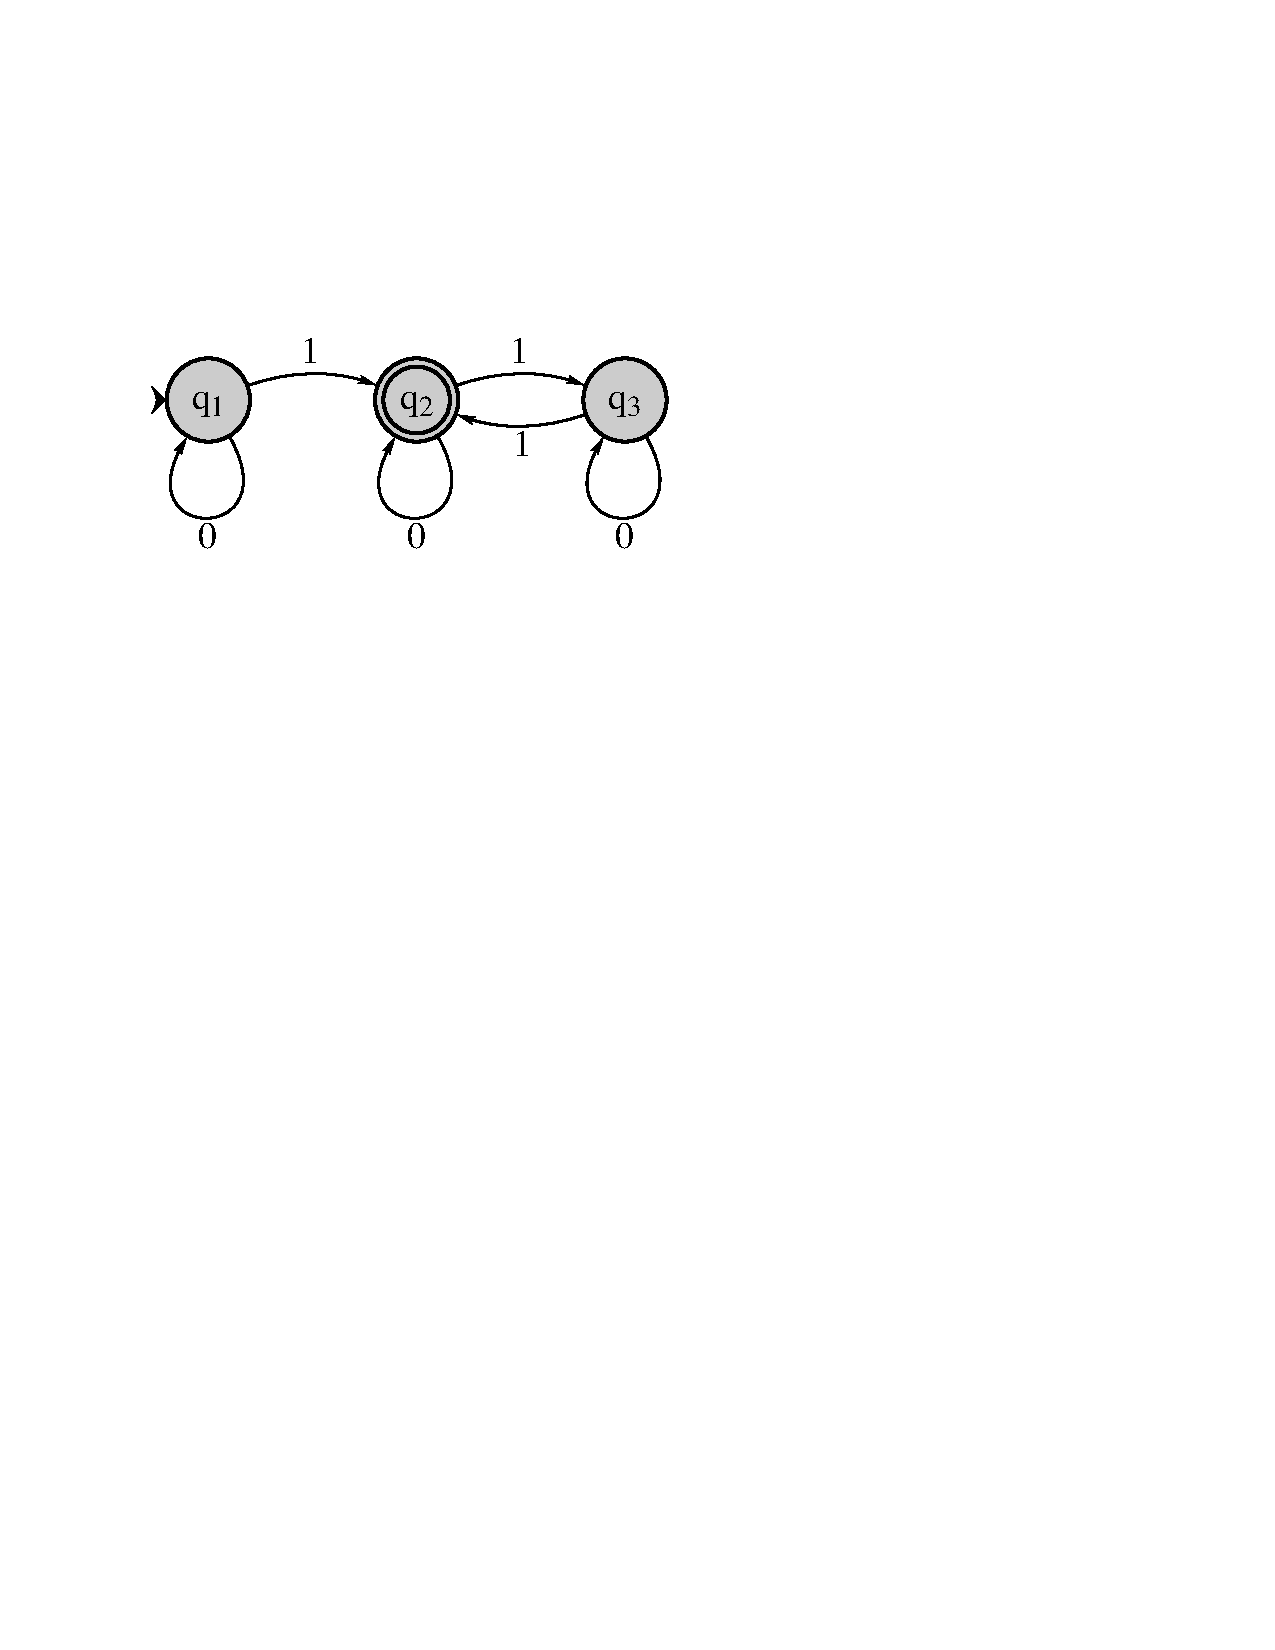
\includegraphics{automin1.pdf}}
\end{center}
\caption{A simple finite automaton}
\label{autom}
\end{figure}
         % Chapter 7, chap7.tex contains an
                        % example of figs and tables and inclusion of pdf.

%%%%%%%%%%%%%%%%%%%%
% Concluding Pages %
%%%%%%%%%%%%%%%%%%%%%%%%%%%%%%%%%%%%%%%%%%%%%%%%%%%%%%%%%%%%%%%%%%%%%%%%%%%%%%%%

% Bibliography or References, REQUIRED

% If using bibtex, create or modify the refs.bib file
% and use (uncomment) the following three lines.
%\bibliographystyle{plain}     %You may prefer \bibliographystyle{alpha}
%\addcontentsline{toc}{chapter}{\bibname}
%\bibliography{refs}         

% If using the ``thereference'' environment instead, modify the ref.tex file
% and use the following line
% ref.tex {References}

\addcontentsline{toc}{chapter}{References}
\begin{thereferences}{99}

\bibitem{Cook1971}
S.~Cook,
 ``The complexity of theorem-proving procedures,''
 {\it Proceedings of the 3rd ACM Symposium on Theory of Computing},
 Shaker Heights, Ohio, 1971, pp.~151--158.

\bibitem{Garey1979}
M.~R.~Garey and D.~S.~Johnson,
 {\it Computers and Intractability: A Guide to the Theory of\/
 {\rm NP}-Completeness},
 W.~H.~Freeman, San Francisco, 1979.

\bibitem{Karp1972}
R.~Karp,
 ``Reducibility among combinatorial problems,''
 in: R.~Miller and J.~Thatcher (eds.),
 {\it Complexity of Computer Computations},
 Plenum Press, New York, 1972, pp.~85--103.

\bibitem{Kearfott1996}
R.~B.~Kearfott and V.~Kreinovich (eds.),
 {\it Applications of Interval Computations},
 Kluwer Academic Publishers, Norwell, MA, 1996.

\bibitem{Kreinovich1993}
V.~Kreinovich, A.~V.~Lakeyev and S.~I.~Noskov,
 ``Optimal solution of interval linear systems is intractable (NP-hard),''
 {\it Interval Computations},
 1993, No. 1, pp. 6--14.

\bibitem{Kreinovich1996a}
 V.~Kreinovich, A.~V.~Lakeyev and J.~Rohn ,
 ``Computational complexity of interval algebraic problems: some are feasible
 and some are computationally intractable: a survey,''
 in: G.~Alefeld and A.~Frommer (eds.),
 {\it Scientific Computing and Validated Numerics},
 Akademie-Verlag, Berlin, 1996, pp.~293--306.

\bibitem{Kreinovich1996b}
 V.~Kreinovich, A.~V.~Lakeyev, J.~Rohn and P.~Kahl,
 {\it Feasible? Intractable? On Computational Complexity of Data Processing
 and Interval Computations},
 Kluwer Academic Publishers, Norwell, MA, 1996 (to appear).

\bibitem{Kulisch1981}
U.~Kulisch and W.~L.~Miranker,
 {\it Computer Arithmetic in Theory and Practice},
 Academic Press, NY, 1981.

\bibitem{Lakeyev1995}
A.~V.~Lakeyev and V.~Kreinovich,
 ``If input intervals are small enough, then interval computations are almost
 always easy,''
 {\it Reliable Computing},
 Supplement (Extended Abstracts of APIC'95: International Workshop on 
 Applications of Interval Computations),
 1995, pp. 134--139.

\bibitem{Levin1973}
L.~Levin,
 ``Universal sequential search problems,''
 {\it Problems of Information Transmission},
 1973, Vol. 9, No. 3, pp. 265--266.

\bibitem{Moore1959}
R.~E.~Moore,
 ``Automatic error analysis in digital computation,''
 {\it Technical Report LMSD-48421},
 Lockheed Missiles and Space Co., Palo Alto, CA, January 1959.

\bibitem{Moore1966}
R.~E.~Moore,
 {\it Interval Analysis},
 Prentice Hall, Englewood Cliffs, NJ, 1966.

\bibitem{Neumaier1990}
A.~Neumaier,
 {\it Interval Methods for Systems of Equations},
 Cambridge University Press, Cambridge, 1990.

\bibitem{Rabinovich1995}
S.~G.~Rabinovich,
 {\it Measurement Errors: Theory and Practice},
 American Institute of Physics, NY, 1995.

\end{thereferences}


% If including appendices, uncomment the following lines,
% adding more includes if needed.
%\StartAppendix
%% Appendix A

\chapter{Batches fabrication and hardness/density measurements details} % Main appendix title

\label{AppendixA} % For referencing this appendix elsewhere, use \ref{AppendixA}

\section{Process parameters and measured hardness/density properties}
\label{ppa}
All manufacturing set values are gathered in table \ref{table:Pparam}. Dimensions of the cubic, cylindrical and parallelepiped specimens are noted in accordance with figure \ref{fig:cc}.\\

 \begin{center}
%\begin{table}[ht]
\setlength\LTleft{-0.7in}
%\setlength\LTright{-1in}
\begin{landscape}
\begin{savenotes}

\begin{longtable}{@{\extracolsep{\fill}}*{12}{|c}|@{}}
    \hline
  Batch name & Contour & Type & Dimensions [mm] &Specimen name & $\frac{P}{P_{max}} [-]$ & $v_s [\frac{mm}{s}]$ & $E_d [\frac{J}{mm^3}]$ & $H_v [HV]$ & $\rho_{rel}$ \footnote{Measured by RODIA [\%].} & $\rho_{a,rel}$ \footnote{Measured by HW (AB specimens) [\%].} & $\rho_{a,rel}$ \footnote{Measured by HW (polished specimens) [\%].} \\
  \hline
  \hline
  \endfirsthead
\multicolumn{12}{c}%
{\tablename\ \thetable\ -- \textit{Continued from previous page}} \\
\hline
Batch name & Contour & Type & Dimensions [mm] &Specimen name & $\frac{P}{P_{max}} [-]$ & $v_s [\frac{mm}{s}]$  & $E_d [\frac{J}{mm^3}]$ & $H_v [HV]$ & $\rho_{rel}$  & $\rho_{a,rel}$  & $\rho_{a,rel}$ \\
\hline
\endhead

\hline \multicolumn{12}{c}{\textit{Continued on next page}} \\
\caption[Manufacturing process parameters]{Manufacturing process parameters}
\label{table:Pparam}

\endfoot
\hline
\endlastfoot

  X200-171024 & No & Cubic & L=10& 1 & 0.85 & 900 & 86.13 &135.9 & - &99.24 &-\\
  & &   & & 2 &  & 1000 & 77.52 &133.7 &- &99.08 &-\\
  & &   & & 3&  & 1059& 73.20 &135.5 & -&99.00 &-\\
  & &  & & 4&  & 1500&51.68 &137.3 & -&99.38 &-\\
  & &  & & 5& 1 & 900&101.33 &131.3 &- &98.81 &-\\
  & &  & & 6&  & 1059&86.12 &132.7 & -&98.83 &-\\
  & & & & 7 & 0.75 & 1200& 57 &137.3 &- &99.49 &-\\
  & & & & 7a & & & &137.9 & -&99.33 &-\\
  & & & & 7b & & & &137.9 &- &99.45 &-\\
  & & & & 8& & 900&76 &135.5 &- &99.23 &-\\
    & & & & 8a & & & & 133.7& -&98.77 &-\\
      & & & & 8b & & & & 136.1& -&99.23 &-\\
\hline  
  X200-180109 & No&Cubic & L=10 & 7c & 0.75 &1200 &57 &141.0 &99.77 &99.33 &99.77\\
  & & & & 7d & && &138.6  &- &99.45 &-\\
  & & & & 7e & & & &140.0 &- &99.44 & -\\
    & & & & 7n & & & &141.4 &- &99.45 &-\\
  & & & & 7g & & & &139.4 & -&99.50 &-\\
  & & & & 7h & & & &139.2 &99.51 &99.52 &99.32\\ 
  & & & & 7i & & & &140.3 &- &99.48 &-\\        
  & & & & 7j & & & &140.9 & -&99.48 &-\\        
  & & & & 7k & & & &140.6 & -&99.37 &-\\        
  & & & & 7l & & & &139.8 & -&99.38 &-\\        
  & & & & 7m & & & &139.0 &99.65 &99.29 &99.48\\      
  & & & & 7n & & & &140.0 &99.51 &99.24 &99.48\\      
  & & & & 7o & & & &138.7 &99.52 &99.49 &99.49\\
  & & & & 7p & & & &140.6 & -&99.37 &-\\
  & & & & 7q & & & &139.0 & -&99.31 &-\\                    
  & & & & 8c& & 900 & 76 &139.4 &- &99.27 &-\\
  & & & & 8d & & & &138.8 & -&99.20 &-\\
  & & & & 8e & & & &138.0 &- &99.29 &-\\
  & & & & 8f & & & &138.3 & -&99.50 &-\\
  & & & & 8g & & & &138.2 & -&99.37 &-\\
  & & & & 8h & & & &139.5 & -&99.51 &-\\
  & & & & 8i & & & &134.6 &- &99.18 &-\\
  & & & & 8j & & & &138.0 & -&99.44 &-\\
  & & & & 8k & & & &138.0 &- &99.41 &-\\  
  & & & & 8l & & & &136.5 & -&99.39 &-\\
  & & & & 8m & & & &139.0 & -&99.31 &-\\
  & & & & 8n & & & &140.4 &- &99.29 &-\\
  & & & & 8o & & & &138.5 &- &99.54 &-\\     
  & & & & 8p & & & &138.7 & -&99.35 &-\\
  & & & & 8q & & & &138.7 & -&99.43 &-\\        
\hline  
  X200-180220 & No & Cubic & L=5 & TT150-2 & 0.75 & 1200 & 57 & & & -&-\\
  & &  & & TT200-2 &  & & & & & -&-\\
  & &  & & TT300-2 &  & & & & &- &-\\
  & &  & & TT300-2-plaque &  & & & & &- &-\\
  & &  & & TT150-2-real &  & & & & &- &-\\
  & &  & & TT200-2-real &  & & & & &- &-\\
  & &  & & TT225-2-real (?) &  & & &116.6 & &- &-\\
  & &  & & TT250-2-real &  & & & & &- &-\\
  & &  & & TT300-5min-real &  & & &101.8 & & -&-\\  
  & &  & & TT300-2-real &  & & & & & - &-\\
\hline  
  X200-180222 & No & Cubic & L=10 &12& 0.75 & 1200 & 57 & - &- &98.30 &-\\
  & &  & &13 &  & & &- &- &98.90 &-\\
\hline  
  X200-180228  & Yes & Cylindrical & D=6, H=2 &1 & 0.75 & 1200 &57 &- &98.87 &- &-\\
  & &  &  & 2&  & & &- &99.23 &- &-\\
  & &  &  & 3 &  & & &- &- &- &-\\
\hline  
  X200180313 & Yes & Cylindrical & D=6, H=10&1& 0.75 & 1200 &57 &- &99.74 &- &-\\
    & &    & &2 & & & &- &99.77 &- &- \\
    & &  &D=12, H=10 &3& & & &- &99.75 & -& -\\
    & & & &4 & & & &- &99.73 &- &-\\
    & No & Parallelepiped & H=10, W=40, L=120 & ??? & & & &- &- &- &-\\
        &  & & & ??? & & & &- &- &- &-\\
\hline  
  X200-180315 & No & Parallelepiped & H=10, W=40, L=115& ??? & 0.75 & 1200 &57 &- &- &- &-\\
  \hline
  X200-180319  & No & Cubic & L=10 & cub 1 & 0.75 & 1200 &57 &139.5 & 99.88&- &99.90\\
  & &  & & cub 2 & & & &140.8 &99.81 &- &99.80\\
  & &  & & cub 3 & & & &140.1 &99.79 &- &99.61\\
  & & & & cub 4 & & & &138.6 &99.85 &- &99.77\\
  & & & & cub 5 & & & &139.9 &99.87 &- &99.68\\
  & & &  L=5& TT300-1-real &  & & & & &- &-\\ 
  & Yes &  Cylindrical & D=6, H=10&cyl 1   &  & & &- &99.85 &- &-\\
    & &  & &cyl 2 & & & & -&99.92 &- &-\\
    & &  & D=12, H=10 &cyl 3 & & & &- &99.85 &- &-\\
    & &  &  &cyl 4  & & & &- &99.82 &- &-\\
 & No & Parallelepiped & H=10, W=40, L=120 & ??? & & & & & & &\\ 
    \hline 
X200-180417 & Yes & Tensile & (see section \ref{MMFPP}) & 1, ..., 24 & 0.75 &1200 &57 & -& -& -&-\\
& &  & & 25 & && &138.0 &99.80 &- &-\\
& No &  & & 26, 27, 28 & && &- &- &- &-\\
&  & Cubic & L=10 & A & & & &135.9 &99.64 &- &99.44\\
&  & & & B & && &138.0 & 99.70& -&99.54\\
&  & & & C & && & 134.1&99.67 &- &99.44\\
\end{longtable}
\end{savenotes}
\end{landscape}
%\end{table}
 \end{center}

\section{Specimens positioning, fabrication orders and sintering times}
\label{mda}
\subsection{Batch X200-171024}

\begin{figure}[ht]
\centering
\noindent\makebox[\textwidth]{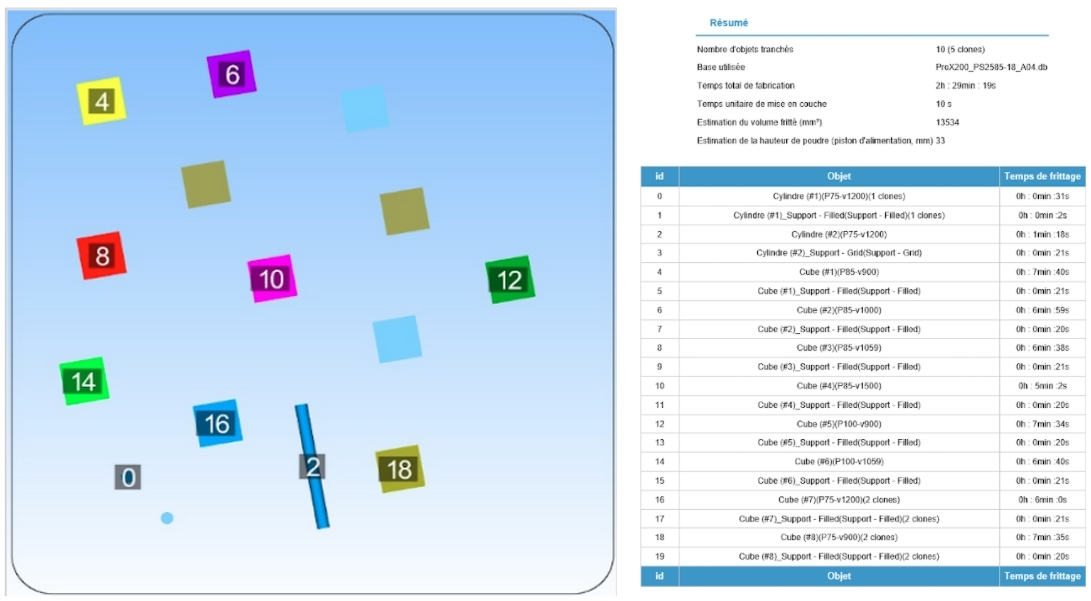
\includegraphics[scale=0.58]{Images/171024-cad}}
\decoRule
\caption[Specimens positions, order of fabrication and sintering times for batch X200-171024]{Specimens positions, order of fabrication and sintering times for batch X200-171024}
\label{fig:171024-cad}
\end{figure}

\begin{figure}[ht]
\centering
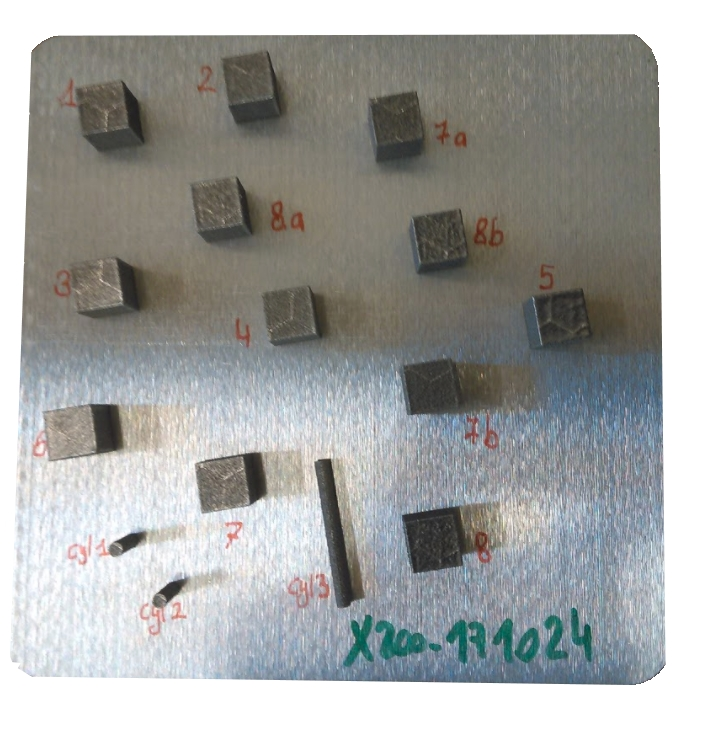
\includegraphics[scale=0.45]{Images/171024-real}
\decoRule
\caption[Photography of the manufacturing plate after completion of the fabrication of batch X200-171024]{Photography of the manufacturing plate after completion of the fabrication of batch X200-171024}
\label{fig:171024-real}
\end{figure}


\subsection{Batch X200-180109}

\begin{figure}[ht]
\centering
\noindent\makebox[\textwidth]{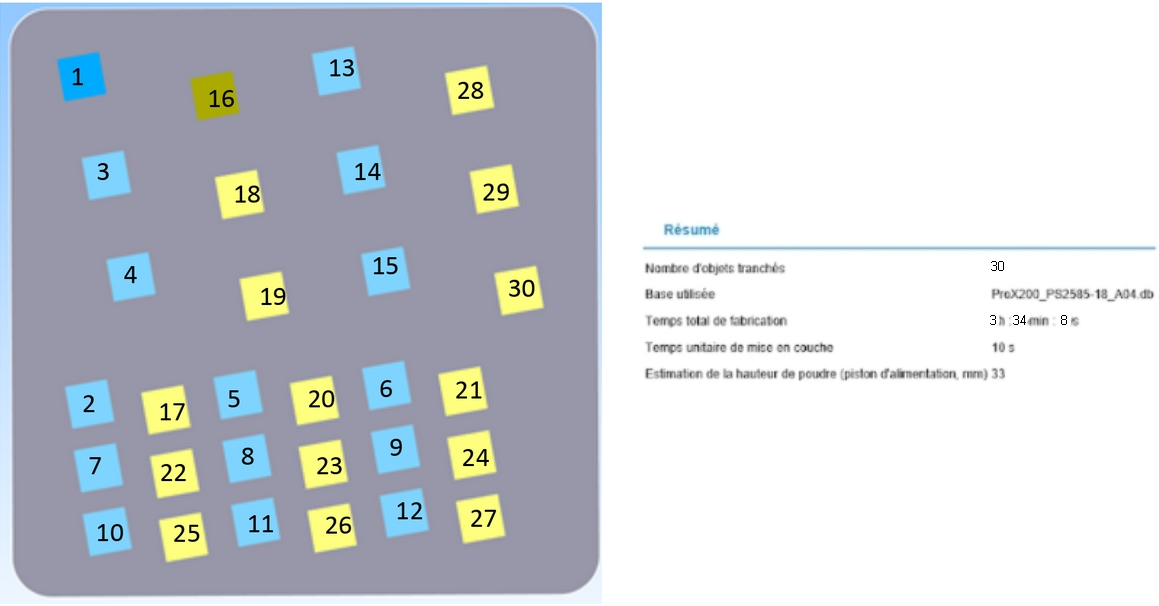
\includegraphics[scale=0.58]{Images/180109-cad}}
\decoRule
\caption[Specimens positions, order of fabrication and sintering times for batch X200-180109]{Specimens positions, order of fabrication and sintering times for batch X200-180109}
\label{fig:171024-cad}
\end{figure}

\begin{figure}[ht]
\centering
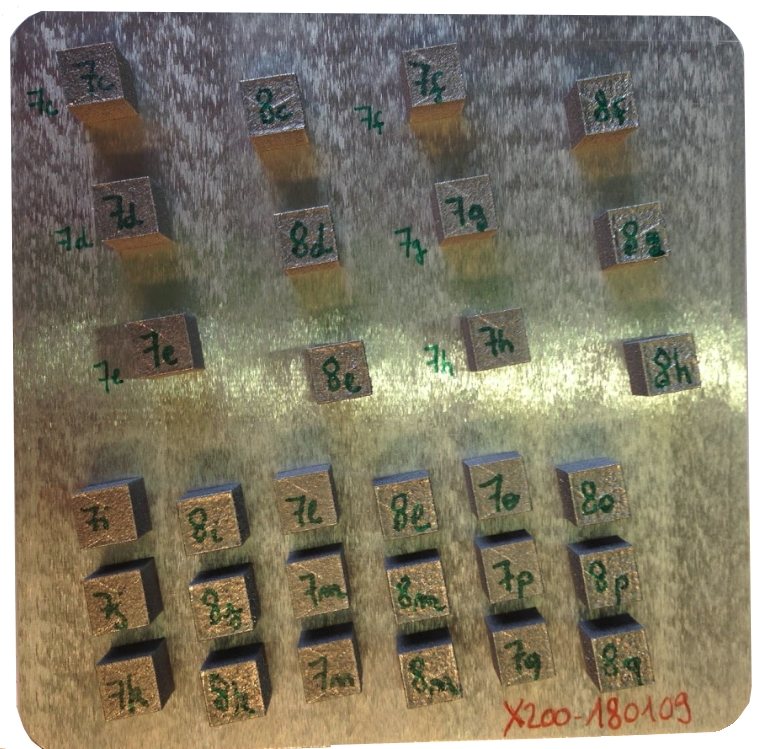
\includegraphics[scale=0.45]{Images/180109-real}
\decoRule
\caption[Photography of the manufacturing plate after completion of the fabrication of batch X200-180109]{Photography of the manufacturing plate after completion of the fabrication of batch X200-180109}
\label{fig:180109-real}
\end{figure}

\subsection{...Other batches}         % Example of how to include an appendix

% vitae.tex (Curriculum Vitae)

\addcontentsline{toc}{chapter}{Curriculum Vitae}
\chapter*{Curriculum Vitae}

Patrick Thor Kahl was born on July 12, 1961. The first son of Ulf Thor Gustav 
Kahl and Carolyn Kahl, he graduated from Coronado High School, El Paso, Texas, 
in the spring of 1979.  He entered Auburn University in the fall of 1979, and,
in the spring of 1982, The University of Texas at El Paso.  In 1985 he joined
the United States Navy where he served for eight years, most of it aboard the
submarine USS Narwhal (SSN671).  In the fall of 1993, after being honorably
discharged from the navy, Patrick resumed his studies at The University of
Texas at El Paso.  While pursuing his bachelor's degree in Computer Science he
worked as a Teaching Assistant, and as a programmer at the National
Solar Observatory at Sunspot, New Mexico.  He received his bachelor's degree
in Computer Science in the summer of 1994.

In the fall of 1994, he entered the Graduate School of The University of Texas 
at El Paso.  While pursuing a master's degree in Computer Science he worked as 
a Teaching and Research Assistant, and as the Laboratory Instructor for the
1995 Real-Time Programming Seminar at the University of Puerto Rico,
Mayag\"{u}ez Campus.  He was a member of the Knowledge Representation Group
and the Rio Grande Chapter of the Association for Computing Machinery.

\medskip

\noindent
Permanent address: 6216 Sylvania Way

\noindent
\hspace{1.42in}
El Paso, Texas 79912-4927

\vfill

% The following is no longer needed when typed by the author.
%\noindent
%This thesis was typed by <name of typist>.


         % Curriculum Vitae      REQUIRED

%%%%%%%%%%%%%%%%%%%%%%%%%%%%%%%%%%%%%%%%%%%%%%%%%%%%%%%%%%%%%%%%%%%%%%%%%%%%%%%%

\end{document}
